\documentclass{article}

% Table of contents formatting
\usepackage{tocloft}

\renewcommand\cftsecfont{\normalfont}
\renewcommand\cftsecpagefont{\normalfont}
\renewcommand{\cftsecleader}{\cftdotfill{\cftsecdotsep}}
\renewcommand\cftsecdotsep{\cftdot}
\renewcommand\cftsubsecdotsep{\cftdot}
\cftsetindents{section}{0em}{3em}
%\cftsetindents{subsection}{1em}{3em}

\usepackage{graphicx}
\usepackage{wrapfig}
\usepackage{subcaption}
\usepackage[margin=1in]{geometry}
\usepackage{amsmath}
\usepackage{siunitx}
\usepackage{booktabs}
\usepackage[export]{adjustbox}
\newcommand{\colormap}{jet}  % colorbar to use
\usepackage{cleveref}
\usepackage{booktabs}
\usepackage{gensymb}
\usepackage{float}
\usepackage{xr}
\usepackage{array}
\usepackage{multirow}

\newcolumntype{P}[1]{>{\centering\arraybackslash}p{#1}}
\newcolumntype{M}[1]{>{\centering\arraybackslash}m{#1}}
\newcommand{\PreserveBackslash}[1]{\let\temp=\\#1\let\\=\temp}
\newcolumntype{C}[1]{>{\PreserveBackslash\centering}p{#1}}
\newcolumntype{R}[1]{>{\PreserveBackslash\raggedleft}p{#1}}
\newcolumntype{L}[1]{>{\PreserveBackslash\raggedright}p{#1}}

\externaldocument[M-]{Final_Draft}

\renewcommand{\thefigure}{S\arabic{figure}}
\renewcommand{\thesection}{S\arabic{section}}
\renewcommand{\thepage}{S\arabic{page}}
\renewcommand{\thetable}{S\arabic{table}}

\title{Supplemental Material: Capturing Subdiffusive Solute Dynamics and 
Predicting Selectivity in Nanoscale Pores with Time Series Modeling.}
\author{Benjamin J. Coscia \and Michael R. Shirts} 

\begin{document}

  \maketitle
  \tableofcontents
  \graphicspath{{./supporting_figures/}}
  \bibliographystyle{ieeetr}
  
  \newpage  
  
  \section{Setup and analysis scripts}\label{section:python_scripts}

  All python and bash scripts used to set up systems and conduct post-simulation trajectory
  analysis are available online at \texttt{https://github.com/shirtsgroup/LLC\_Membranes}.
  Documentation for the \texttt{LLC\_Membranes} repository is available at
  \texttt{https://llc-membranes.readthedocs.io/en/latest/}. Table~\ref{table:python_scripts}
  provides more detail about specific scripts used for each type of analysis performed in
  the main text.

  \begin{table}[htb!]
  \centering
  \newcolumntype{A}{ >{\centering\arraybackslash} m{2.5in} }
  \newcolumntype{B}{ >{\centering\arraybackslash} m{0.5in} }
  \newcolumntype{C}{m{3in}}
  \begin{tabular}{|A|B|C|}
  \hline
  \textbf{Script Name} & \textbf{Section} & ~~~~~~~~~~~~~~~~~~~~~\textbf{Description} \\
  \hline

  % mimic this
  \texttt{/setup/parameterize.py}            & 2.1 & Parameterize liquid crystal monomers and solutes with GAFF \\ \hline
  \texttt{/setup/build.py}                   & 2.1 & Build simulation unit cell \\ \hline
  \texttt{/setup/place\_solutes\_pores.py}   & 2.1 & Place equispaced solutes in the pore centers of a unit cell \\\hline
  \texttt{/setup/equil.py}                   & 2.1 & Equilibrate unit cell and run production simulation \\\hline
  \texttt{/analysis/solute\_partitioning.py} & 2.1 & Determine time evolution of partition of solutes between pores and tails \\\hline
  \texttt{/timeseries/msd.py}                & 2.2 & Calculate the mean squared displacement of solutes \\\hline
  \texttt{/analysis/sfbm\_parameters.py}     & 2.2 & Get subordinated fractional Brownian motion parameters by fitting to a solute's dwell and hop length distributions and positional autocorrelation function. \\\hline
  \texttt{/timeseries/ctrwsim.py}            & 2.2 & Generate realizations of a continuous time random walk with the user's choice of dwell and hop distributions \\\hline
  \texttt{/timeseries/forecast\_ctrw.py}     & 2.2 & Combines classes from \texttt{sfbm\_parameters.py} and \texttt{ctrwsim.py} to parameterize and predict MSD in one shot. \\\hline
  \texttt{/analysis/ Markov\_state\_dependent\_dynamics.py} & 2.3 & Identify frame-by-frame state of each solute, construct a transition matrix and simulate realizations of the MSDDM model. \\\hline
  \texttt{/timeseries/mfpt\_pore.py}          & 2.4 & Simulate mean first passage time distributions using the AD approach. \\\hline 
  \end{tabular}

  \caption{The first column provides the names of the python scripts available in
  the \texttt{LLC\_Membranes} GitHub repository that were used for system setup and
  post-simulation trajectory analysis. Paths preceding script names are relative to the
  \texttt{LLC\_Membranes/LLC\_Membranes} directory. The second column lists the section in the main
  text where the output or usage of the script is first described. The third column
  gives a brief description of the purpose of each script.
  }~\label{table:python_scripts}

  \end{table}
  
  \newpage
  
  \section{Solute Equilibration}\label{section:equilibration}
  
  We collected all data used for model generation after the solutes were 
  equilibrated. We assumed a solute to be equilibrated when the partition of
  solutes in and out of the pore region stopped changing. The pore region is
  defined as within 0.75 nm of the pore center. We've plotted the partition
  versus time in Figure~\ref{fig:equilibration} and indicated the chosen
  equilibration time points. 
  
  %Note that the partition of acetic acid appears
  %to be oscillating slowly. We do not expect the system to plateau on a
  %reasonable time scale, so we settled for including a complete oscillation.
  
  \begin{figure}[hb]
  \centering
  \begin{subfigure}{0.45\textwidth}
  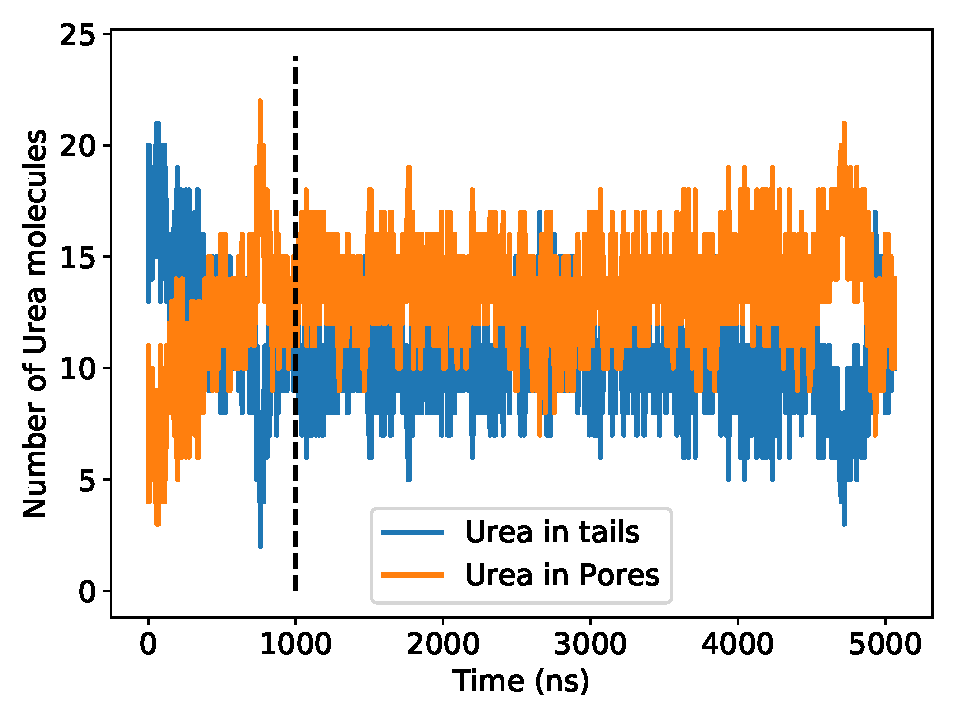
\includegraphics[width=\textwidth]{URE_equilibration.pdf}
  \caption{}\label{fig:URE_equilibration}
  \end{subfigure}
  \begin{subfigure}{0.45\textwidth}
  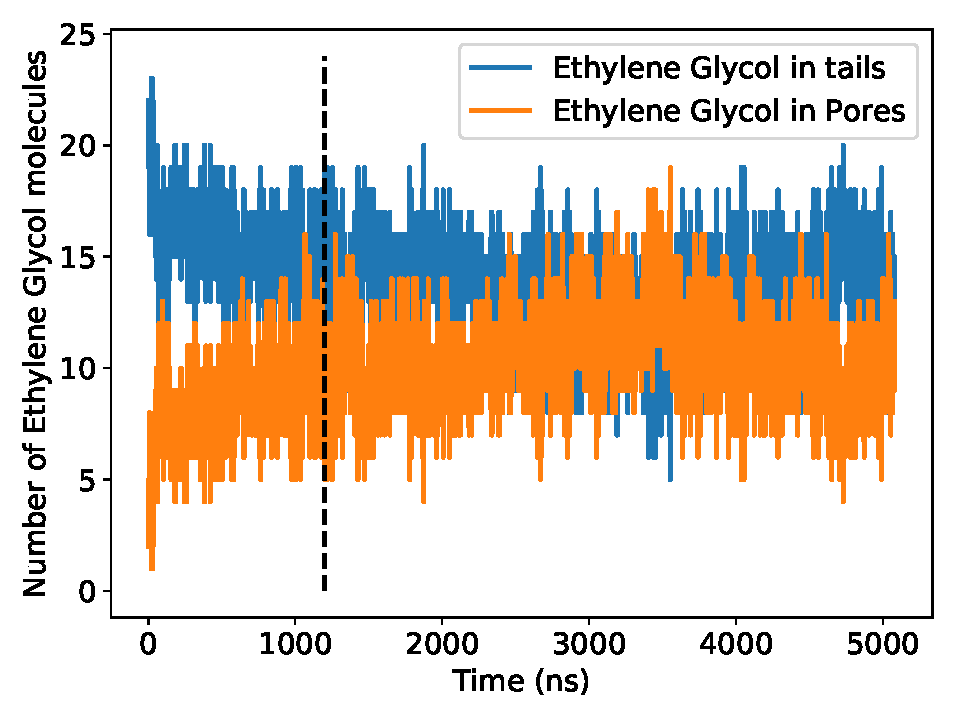
\includegraphics[width=\textwidth]{GCL_equilibration.pdf}
  \caption{}\label{fig:GCL_equilibration}
  \end{subfigure}
  \begin{subfigure}{0.45\textwidth}
  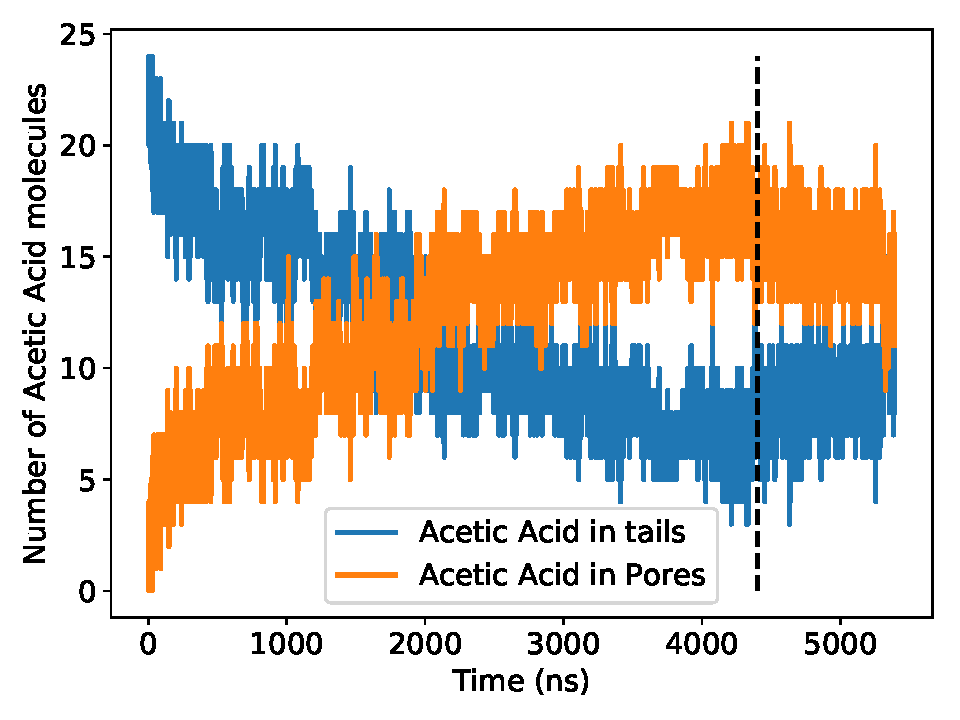
\includegraphics[width=\textwidth]{ACH_equilibration.pdf}
  \caption{}\label{fig:ACH_equilibration}
  \end{subfigure}
  \begin{subfigure}{0.45\textwidth}
  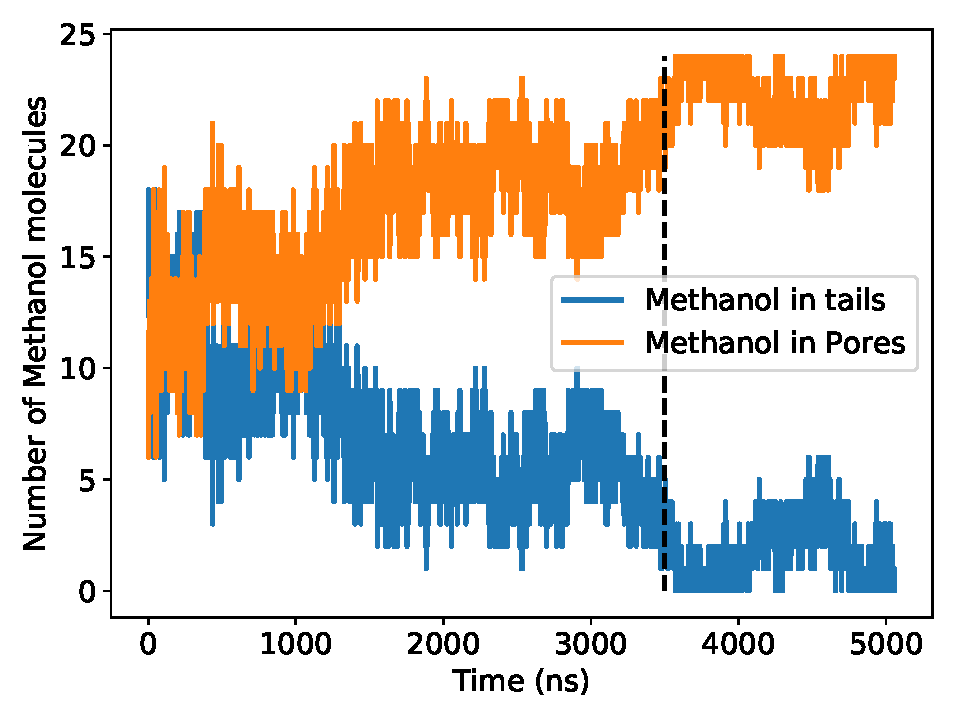
\includegraphics[width=\textwidth]{MET_equilibration.pdf}
  \caption{}\label{fig:MET_equilibration}
  \end{subfigure}
  \caption{We considered a system to be equilibrated when the partition of solutes
  between the tails and pore plateaued. Our chosen equilibration point for each
  solute is indicated by the vertical black dashed line. (a) Urea equilibrates
  the fastest, after 1000 ns. (b) Ethylene glycol equilibrates after 1200 ns 
  (c) The partition of acetic acid appears oscillate slowly. We considered it to be
  equilibrated after 2000 ns. (d) We considered methanol to be equilibrated after
  3500 ns. Methanol nearly completely partitions into the tails.}\label{fig:equilibration}
  \end{figure}

%  \section{Choosing a transport model}\label{section:transport_model_selection}
%
%  We used the toolbox created by Meroz and Sokolov in order to justify our
%  choice of transport model.\cite{meroz_toolbox_2015} The solutes in our systems
%  exhibit anomalous transport properties characteristic of a Continuous Time
%  Random Walk (CTRW). 
%
%  \subsection*{Mean Squared Displacement}
%
%  The general form of a mean squared displacement (MSD) curve is:
%  \begin{equation}
%	\langle x^2(t) \rangle \sim t ^ \alpha
%	\label{eqn:msd}
%  \end{equation}
%  For Brownian motion, $\alpha = 1$ and the MSD is linear. When $\alpha \neq
%  1$, the particle of interest exhibits anomalous diffusion. Values of $\alpha$
%  greater than 1 give rise to superdiffusion, while values of $\alpha$ less than
%  1 give rise to subdiffusion.
%
%  We can calculate the ensemble-averaged MSD curve by averaging the MSDs of
%  each particle trajectory, where each MSD is calculated using:
%  \begin{equation}
%	\delta^2(t) = \| \mathbf{r}(t) - \mathbf{r}(0) \|^2
%	\label{eqn:ensemble_msd}
%  \end{equation}
%  where $\|\cdot\|$ represents the Euclidean norm. 
%
%  The mean squared displacement of solutes in our model is a non-linear
%  function of time, with $\alpha < 1$ which is indicative of anomalous
%  subdiffusion. Figure \ref{fig:msd_power_law}a plots the ensemble-averaged MSD
%  curve for 24 ethanol molecules diffusing in a 10 wt\% water H\textsubscript{II}
%  LLC membrane system. We fit a power law of the form $Ae^{\alpha}$ to the MSD
%  curve. We performed 2000 bootstrap trials by randomly sampling 24 MSD curves
%  with replacement from the 24 total ethanol MSD curves. The bootstrapped average
%  value of $\alpha$ is 0.75 for this system. 
% 
%  \begin{figure}[!htb]
%  \centering
%% Generated with : msd.py -t PR_nojump.xtc -g PR.gro -r ETH -ensemble -power_law -a z -nboot 2000
%% in directory: /home/bcoscia/Documents/Gromacs/Transport/NaGA3C11/ETH/10wt
%  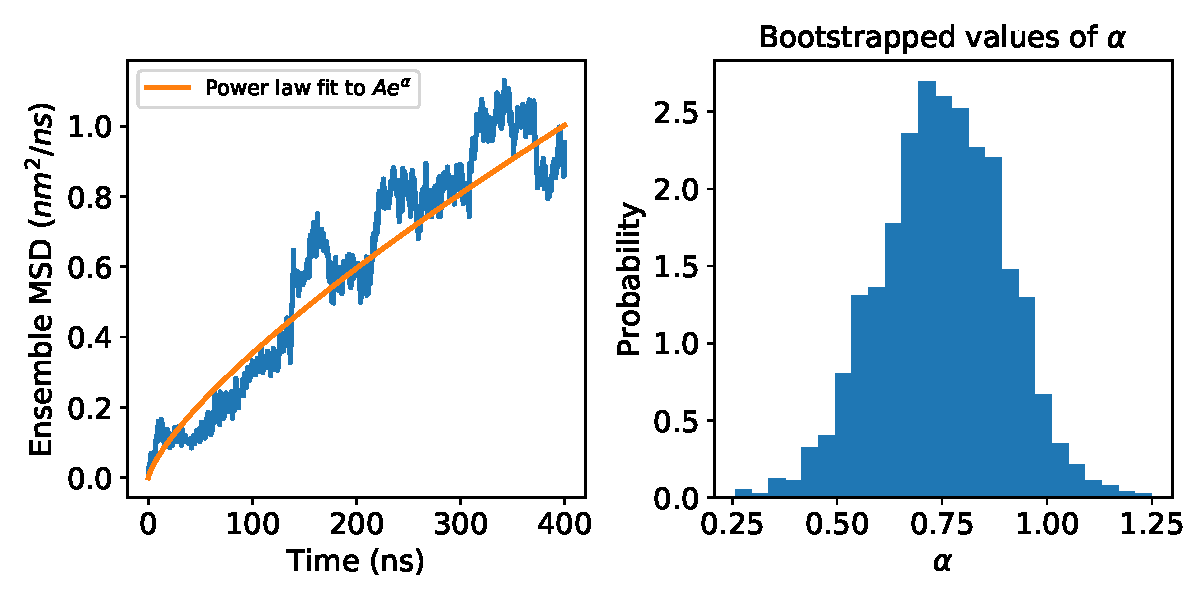
\includegraphics[width=0.8\linewidth]{msd_power_law.pdf}
%  \caption{(a) We fit a curve with the form of Equation~\ref{eqn:msd} to the
%	  ensemble-averaged MSD curve. (b) The average value of $\alpha$, obtained using
%	  fits to MSDs calculated from bootstrapped ensembles, is less than 1 suggesting
%	  that ethanol molecules in our model exhibit subdiffusive
%	  behavior.}\label{fig:msd_power_law}
%  \end{figure}
%
%  \subsection*{Ergodicity}
%
%  The ergodicity of a system can help us narrow down the possible anomalous
%  diffusion mechanisms. In an ergodic system, the time-averaged behavior of an
%  observable should yield the same result as the ensemble average of the same
%  observable. Examples of anomalous diffusion processes that are ergodic include
%  random walks on fractals (RWF) and fractional brownian motion (FBM).
%  Non-ergodic systems generally give rise to CTRWs with the possibility of
%  combination with a RWF and/or FBM.\cite{meroz_toolbox_2015} 
%
%  We tested the ergodicity of our system by comparing the ensemble-averaged
%  and time-averaged MSD curves. We calculated the MSD of each ethanol trajectory
%  using Equation~\ref{eqn:ensemble_msd} and a time-averaged algorithm: 
%  \begin{equation}
%	\delta^2(t) = \dfrac{1}{N-t} \sum_{i=0}^{N-t-1} \| \mathbf{r}(i + t) - \mathbf{r}(i) \|^2
%  \end{equation}
%  where N is the total number of simulation frames, and t represents the length
%  of subinterval or number of frames per subinterval. We averaged the MSD curves
%  from each trajectory in order to create final MSD plots.
%
%  The ethanol molecules exhibit non-ergodic behavior because their
%  time-averaged and ensemble-averaged MSDs do not agree with each other
%  (Figure~\ref{fig:ethanol_msd_comparison}). We validated our analysis using a 1
%  ns simulation of a box of tip3p water molecules. As expected, since the
%  particles exhibit Brownian motion, the time-averaged and ensemble-averaged MSDs
%  agree with each within error (Figure~\ref{fig:water_box_msd_comparison}).
%
%  \begin{figure}[!htb]
%  \centering
%  \begin{subfigure}{0.45\textwidth}
%% Generated with : msd.py -t PR_nojump.xtc -g PR.gro -r ETH -compare -nboot 2000 -a z
%% in directory: /home/bcoscia/Documents/Gromacs/Transport/NaGA3C11/ETH/10wt
%  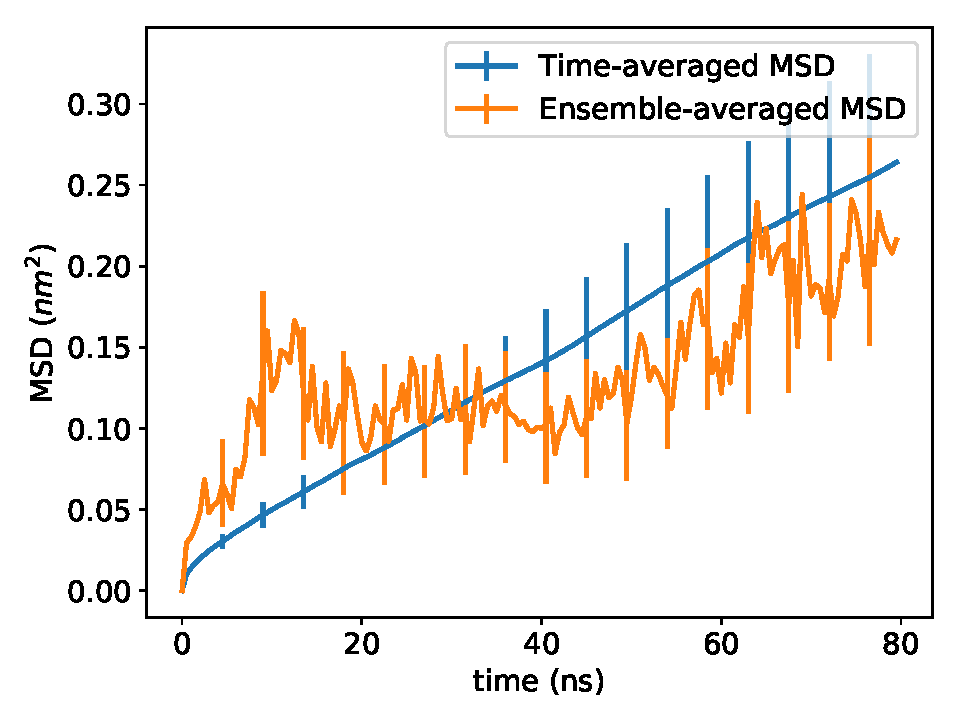
\includegraphics[width=\textwidth]{ethanol_msd_comparison.pdf}
%  \caption{}\label{fig:ethanol_msd_comparison}
%  \end{subfigure} 
%  \begin{subfigure}{0.45\textwidth}
%% Generated with msd.py -t traj_nojump.xtc -g npt.gro -r SOL -compare --fracshow 0.4 -nboot 2000 -a z
%% in directory: /home/bcoscia/Documents/Gromacs/Transport/Solvent/solvent_boxes/pure_water
%  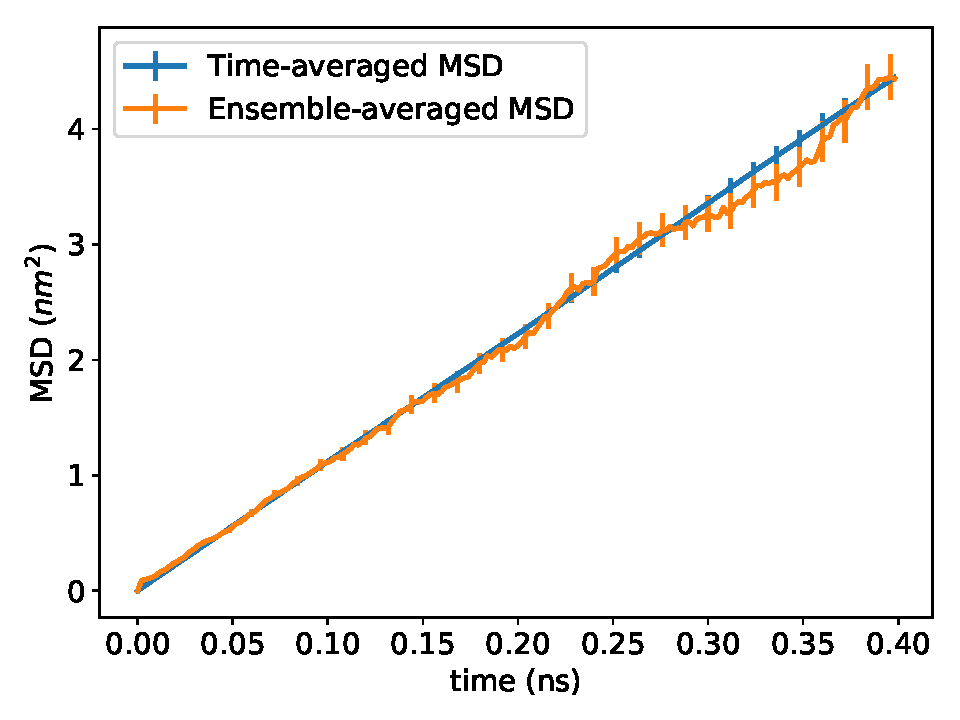
\includegraphics[width=\textwidth]{water_box_msd_comparison.pdf}
%  \caption{}\label{fig:water_box_msd_comparison}
%  \end{subfigure} 
%  \caption{(a) The time-averaged and the ensemble-averaged MSDs for ethanol in
%	  an H\textsubscript{II} nanopore are not in agreement, implying non-ergodicity.
%	  (b) A box of tip3p water molecules is expected to be ergodic and it is shown to
%	  be true here because both MSDs are in agreement. }\label{fig:msd_comparison}
%  \end{figure}

  \newpage
  
  \section{Estimating the Hurst Parameter}\label{section:H_estimate}
  
  We chose to estimate the Hurst parameter, $H$ by a least squares fit to the analytical
  autocorrelation function for fractional Brownian motion (the variance-normalized version 
  of Equation~\ref{M-eqn:fbm_autocorrelation} in the main text):
  
  \begin{equation}
    \gamma(k) = \dfrac{1}{2}\bigg[|k-1|^{2H} - 2|k|^{2H} + |k+1|^{2H}\bigg]
  \label{eqn:fbm_autocorrelation}
  \end{equation}  
  
  In Figure~\ref{fig:hurst_autocorrelation}, we plotted Equation~\ref{eqn:fbm_autocorrelation}
  for different values of $H$. When $H > 0.5$, Equation~\ref{eqn:fbm_autocorrelation} decays
  slowly to zero meaning one needs to study large time lags with high frequency in order to
  accurately estimate $H$ from the data. Fortunately, all of our solutes show anti-correlated
  motion, so most of the information in Equation \ref{eqn:fbm_autocorrelation} is contained
  within the first few lags. 

  % /supporting_figures/hurst_autocorrelation.py
  \begin{figure}
  \centering
  \begin{subfigure}{0.45\textwidth}
  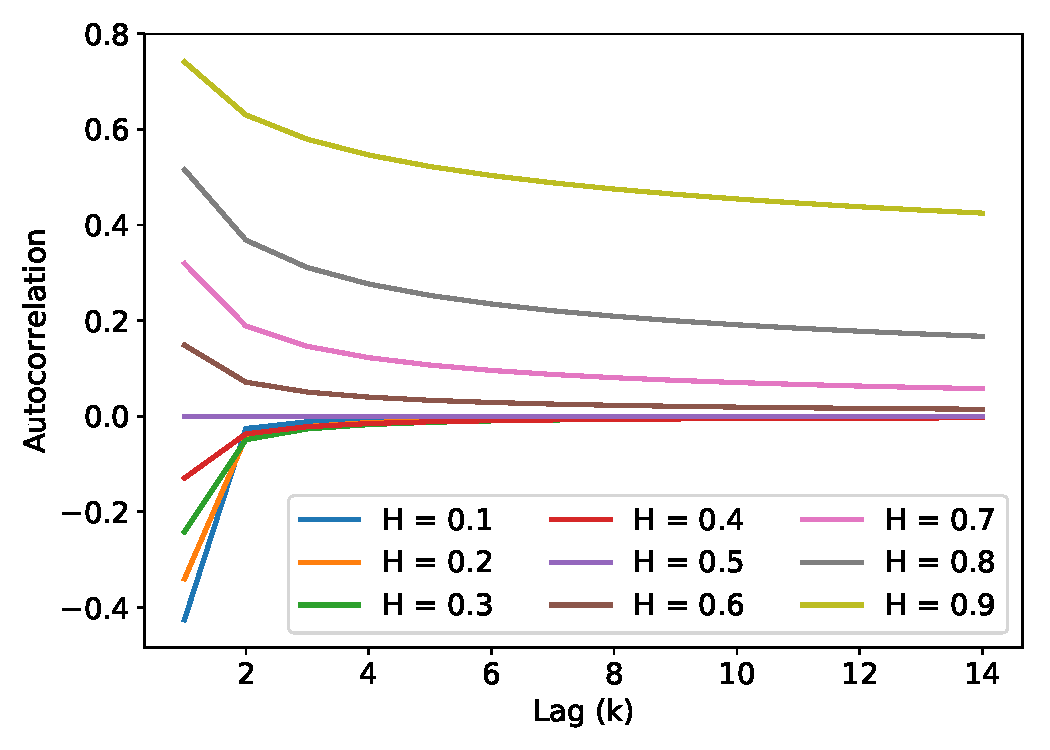
\includegraphics[width=\textwidth]{hurst_autocorrelation.pdf}
  \caption{}\label{fig:hurst_autocorrelation}
  \end{subfigure}
  % supporting_figures/flm_autocov.py
  \begin{subfigure}{0.45\textwidth}
  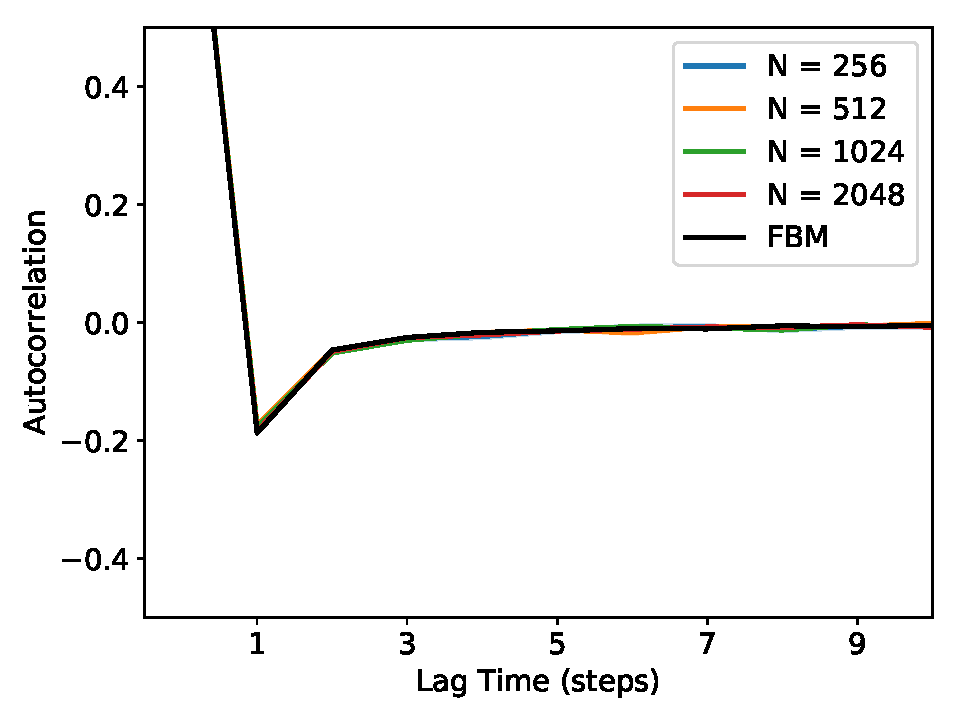
\includegraphics[width=\textwidth]{flm_autocovariance.pdf}
  \caption{}\label{fig:flm_autocorrelation}
  \end{subfigure}  
  \caption{(a) The analytical autocorrelation function of FBM decays to zero faster
  when H $<$ 0.5 compared to when H $>$ 0.5. (b) The autocorrelation function of an 
  FLM process does not change with increasing sequence length (N). It shares the same
  autocorrelation function as fractional Brownian motion (FBM). Note that all lines
  plotted lie on top of each other. All sequences used to make this plot were generated
  using $H$=0.35 and, for FLM, $\alpha$=1.4.}\label{fig:hurst_parameters}
  \end{figure}
  
  The autocovariance function of fractional L\'evy motion is different from fractional
  Brownian motion (see Equations~\ref{M-eqn:fbm_autocorrelation}
  and~\ref{M-eqn:flm_autocovariance} of the main text), but their autocorrelation 
  structures are the same. The autocovariance function of FLM is dependent on the 
  expected value of squared draws from the underlying L\'evy distribution, $E\big[L(1)^2\big]$. 
  This is effectively the distribution's variance, which is undefined for most 
  L\'evy stable distributions due to their heavy tails. As a consequence, one should 
  expect $E\big[L(1)^2\big]$ to grow as more samples are drawn from the distribution
  with the autocovariance function responding accordingly. 
  However, we are only interested in the autocorrelation function. In order to predict
  the Hurst parameter from the autocorrelation function, we must show that it has 
  a well-defined structure and is independent of the coefficient in 
  Equation~\ref{M-eqn:flm_autocovariance} of the main text. In Figure~\ref{fig:flm_autocorrelation}, 
  we plot the average autocorrelation function from an FLM process with an increasing 
  number of observations per generated sequence. For all simulations we set $H$=0.35 
  and $\alpha$=1.4. The variance-normalized autocovariance function, i.e. the autocorrelation
  function, does not change with increasing sequence length. Additionally, the
  autocorrelation function of FBM, with the same $H$, is the same. Therefore we are 
  confident that we can use the same Hurst parameter as an input to both FBM and FLM
  simulations.
  
  \newpage
  
  \section{Simulating Fractional L\'evy Motion}\label{section:sFLM}
  
  % ordered this way to be consistent with mentions in the main text
  \subsection{Truncated L\'evy stable hop distributions}\label{section:truncation}
  
  \textit{Determining where to truncate the hop distribution:} A pure
  L\'evy stable distribution has heavy tails which can lead to arbitrarily
  long hop lengths. Our distribution of hop lengths fits well to a L\'evy
  distribution near the mean, but under-samples the tails. In 
  Figure~\ref{fig:truncation_correction} we compare the empirically 
  measured transition emission distribution of the MSDDM for urea to its maximum likelihood fit to
  a L\'evy stable distribution. The ratio between the two distributions 
  at each bin is nearly 1 close to the center, indicating a near-perfect
  fit, larger than 1 slightly further from the center, suggesting that 
  we slightly over sample intermediate hop lengths, and below 1 far from 
  the center, indicating undersampling of extremely long hop lengths.
  Based on the plot, we chose a cut-off of 1 nm in order to compensate for
  over sampled intermediate hop lengths. We chose the same cut-off for all
  solutes.
  
  \begin{figure}
  \centering
  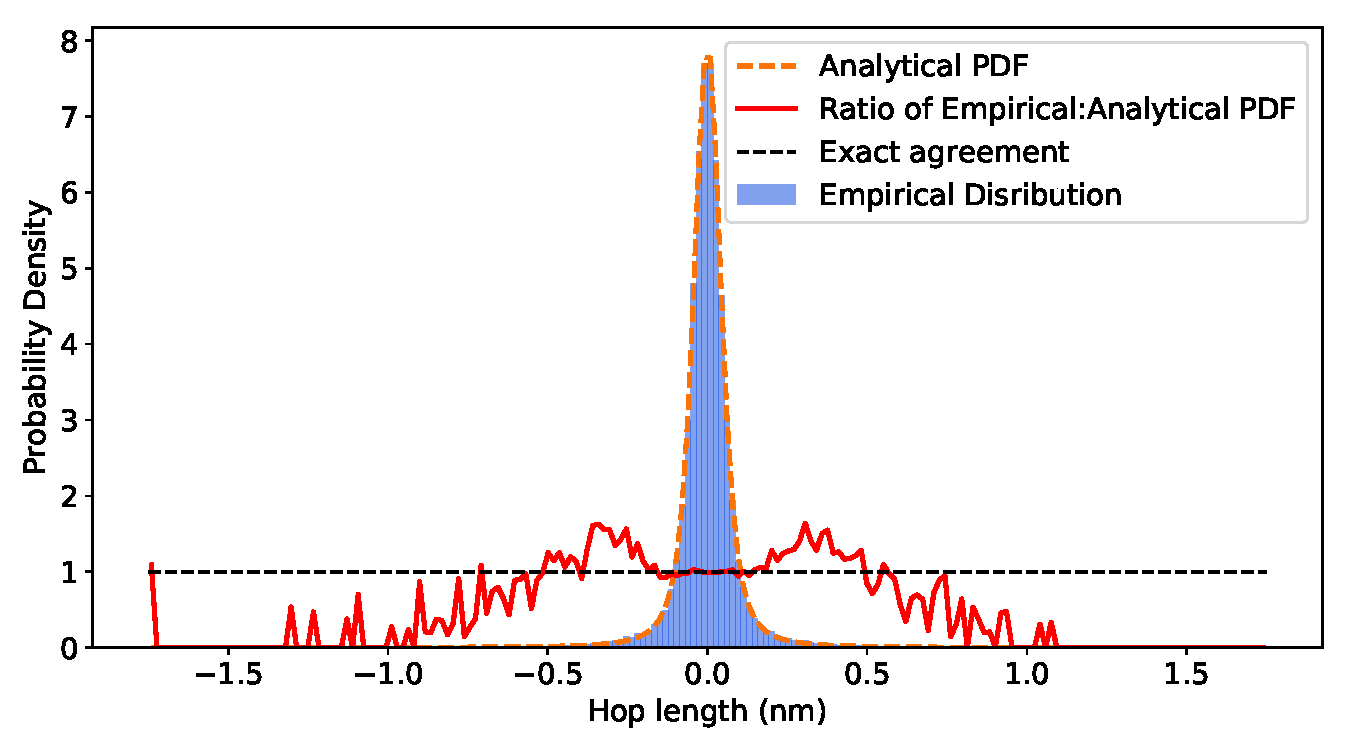
\includegraphics[width=0.75\textwidth]{truncation_cutoff.pdf}
  \caption{The ratio between the empirical and maximum likelihood theoretical
  distribution quantifies the quality of fit as function of hop length. The fit
  is near-perfect close to the mean. Intermediate hop lengths are over sampled, 
  and the tails are undersampled. We used this type of plot to determine the
  appropriate place to truncate the L\'evy stable distributions.}\label{fig:truncation_cutoff}
  \end{figure}
  
  \textit{Generating FLM realizations from a truncated L\'evy distribution:}
  To generate realizations from an uncorrelated truncated L\'evy process, one would
  randomly sample from the base distribution and replace values that are too large
  with new random samples from the base distribution, repeating the process until
  all samples are under the desired cut-off. 
  
  This procedure is complicated by the correlation structure of FLM. At a high level,
  Stoev and Taqqu use Riemann-sum approximations of the stochastic integrals defining
  FLM in order to generate realizations.~\cite{stoev_simulation_2004} They do this efficiently with the help of 
  Fast Fourier Transforms. In practice, this requires one to Fourier transform a zero-padded
  vector of random samples drawn from the appropriate L\'evy stable distribution, multiply
  the vector in Fourier space by a kernel function and invert back to real space. The end
  result is a correlated vector of fractional L\'evy noise.
  
  We are unaware of a technique for simulating truncated FLM, therefore we devised our
  own based on the above discussion. If one is to truncate an FLM process, one can apply
  the simple procedure above for drawing uncorrelated values from the marginal L\'evy 
  stable distribution, \textit{but}, after adding correlation, the maximum drawn value is typically lower than the limit set 
  by the user. Additionally, the shape of the distribution itself changes. Therefore, 
  we created a database meant to correct the input truncation parameter (the maximum desired draw). The database
  returns the value of the truncation parameter that will properly truncate the
  output marginal distribution based on $H$, $\alpha$ and $\sigma$ (the width parameter).
  Figure~\ref{fig:truncation_correction} shows the result of applying our correction.
  Note that generating this database requires a significant amount of simulation and
  still likely doesn't perfectly correct the truncation parameter. The output leads
  to a somewhat fuzzy, rather than abrupt, cut-off of the output distribution. This 
  is likely beneficial since we observe a small proportion of hops longer the chosen
  truncation cut-off. When the cut-off value is close to the L\'evy stable $\sigma$ parameter,
  as it is in our anomalous diffusion models, we observed that the tails of the 
  truncated distribution tend to be undersampled. In order to maintain the distribution's 
  approximate shape up to the cut-off value we recommend ensuring that the cut-off
  value is at least 2 times $\sigma$. However, this may lead to a slight over-prediction
  of the MSD.
  
  \begin{figure}
  \centering
  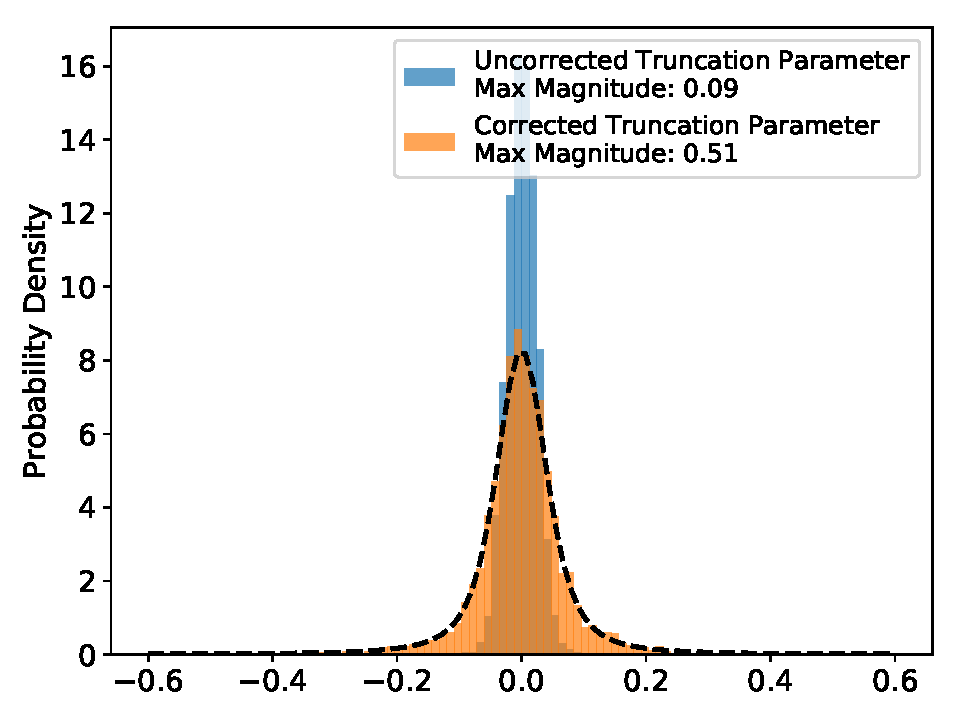
\includegraphics[width=0.5\textwidth]{truncation_correction.pdf}
  \caption{We can accurately truncate the marginal distribution of FLM innovations by
  applying a correction to the input truncation parameter. We generated FLM sequences
  and truncated the initial L\'evy stable distribution (before Fourier transforming) at 
  a value of 0.5. After correlation structure is added, the width of the distribution 
  of fractional L\'evy noise decreases significantly. We corrected the input truncation
  parameter with our database resulting in a distribution close to the theoretical
  distribution (black dashed line) with a maximum value close to 0.5.}\label{fig:truncation_correction}
  \end{figure}
  
  \subsection{Achieving the right correlation structure}\label{section:flm_correlation}
  
  We simulated FLM using the algorithm of Stoev and Taqqu~\cite{stoev_simulation_2004}.
  There are no known exact methods for simulating FLM. As a consequence, passing a
  value of $H$ and $\alpha$ to the algorithm does not necessarily result in the correct
  correlation structure, although the marginal L\'evy stable distribution is correct. 
  We applied a database-based empirical correction in order to use the
  algorithm to achieve the correct marginal distribution and correlation structure.
  
  Stoev and Taqqu note that the transition between negatively and positively correlated
  draws occurs when $H = 1/ \alpha$. When $\alpha=2$, the marginal distribution is 
  Gaussian and the transition occurs at $H=0.5$ as expected from FBM. We corrected 
  the input $H$ so that the value of $H$ measured based on the output sequence equaled
  the desired $H$. We first adjusted the value of $H$ by adding ($1 / \alpha - 0.5$),
  effectively recentering the correlation sign transition for any value of $1 \leq \alpha \leq 2$.
  This correction alone does a good job for input $H$ values near 0.5, but is
  insufficient if one desires a low value of $H$. The exact correction to $H$ is 
  not obvious so we created a database of output $H$ values tabulated as a function
  of input $H$ and $\alpha$ values. Figure~\ref{fig:hurst_correction} demonstrates the
  results of applying our correction. Without the correction, FLM realizations are
  more negatively correlated. This would result in under-predicted mean squared
  displacements when applying the model.
  
  % /supporting_figures/demonstrate_hurst_correction.py
  \begin{figure}
  \centering
  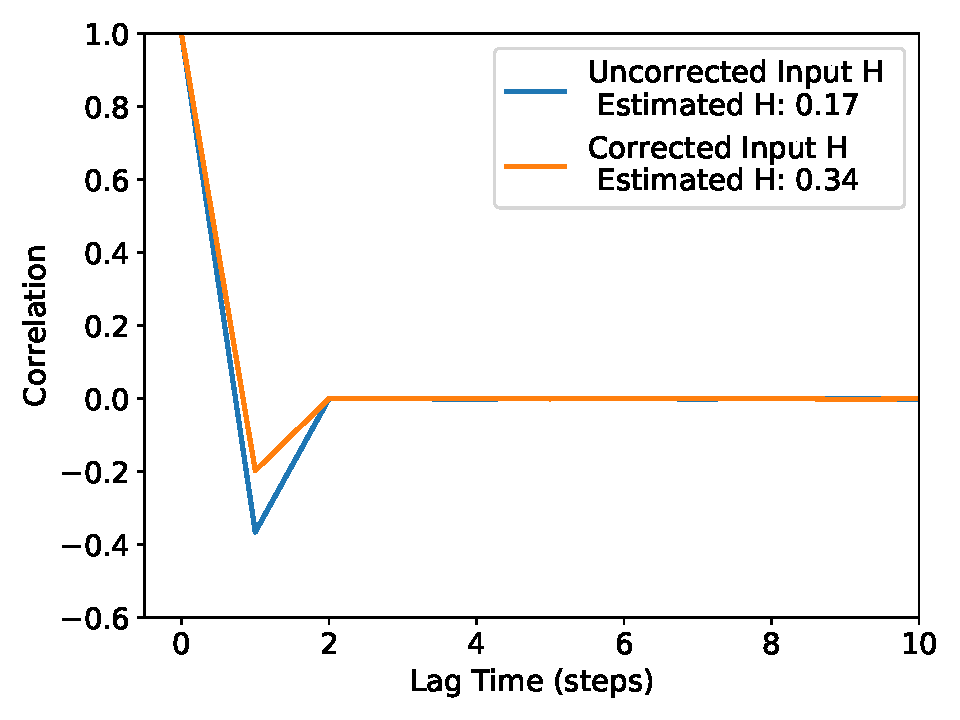
\includegraphics[width=0.5\textwidth]{hurst_correction.pdf}
  \caption{Correcting the Hurst parameter input to the algorithm of Stoev and Taqqu
  results in an FLM process with a more accurate correlation structure. We generated
  sequences with an input $H$ of 0.35. We estimated $H$ by fitting the autocorrelation
  function. Without the correction, $H$ is underestimated, meaning realizations are 
  more negatively correlated than they should be.}\label{fig:hurst_correction}
  \end{figure}
  
  \newpage
  
  \section{Verifying Markovianity}\label{section:markov_validation}
  
  We verified the Markovianity of our transition matrix, $T$, in two ways. First we 
  ensured that the process satisfied detailed balance:
  \begin{equation}
  T_{i,j}P_i(t=\infty) = T_{j,i}P_j(t=\infty)
  \end{equation}
  where $P$ is the equilibrium distribution of states. This implies that the number
  of transitions from state $i$ to $j$ and from state $j$ to $i$ should be equal. Graphical 
  representations of the count matrices show that this is true in Figure~\ref{fig:counts}. 
  
  Second, we ensured that the transition matrix did not change on coarser time scales.
  In Figures~\ref{fig:counts} and~\ref{fig:transitions}, we show that increasing the 
  length of time between samples does not change the properties of the count or
  probability transition matrices.
  
  \begin{figure}
  \centering
  \begin{subfigure}{\textwidth}
  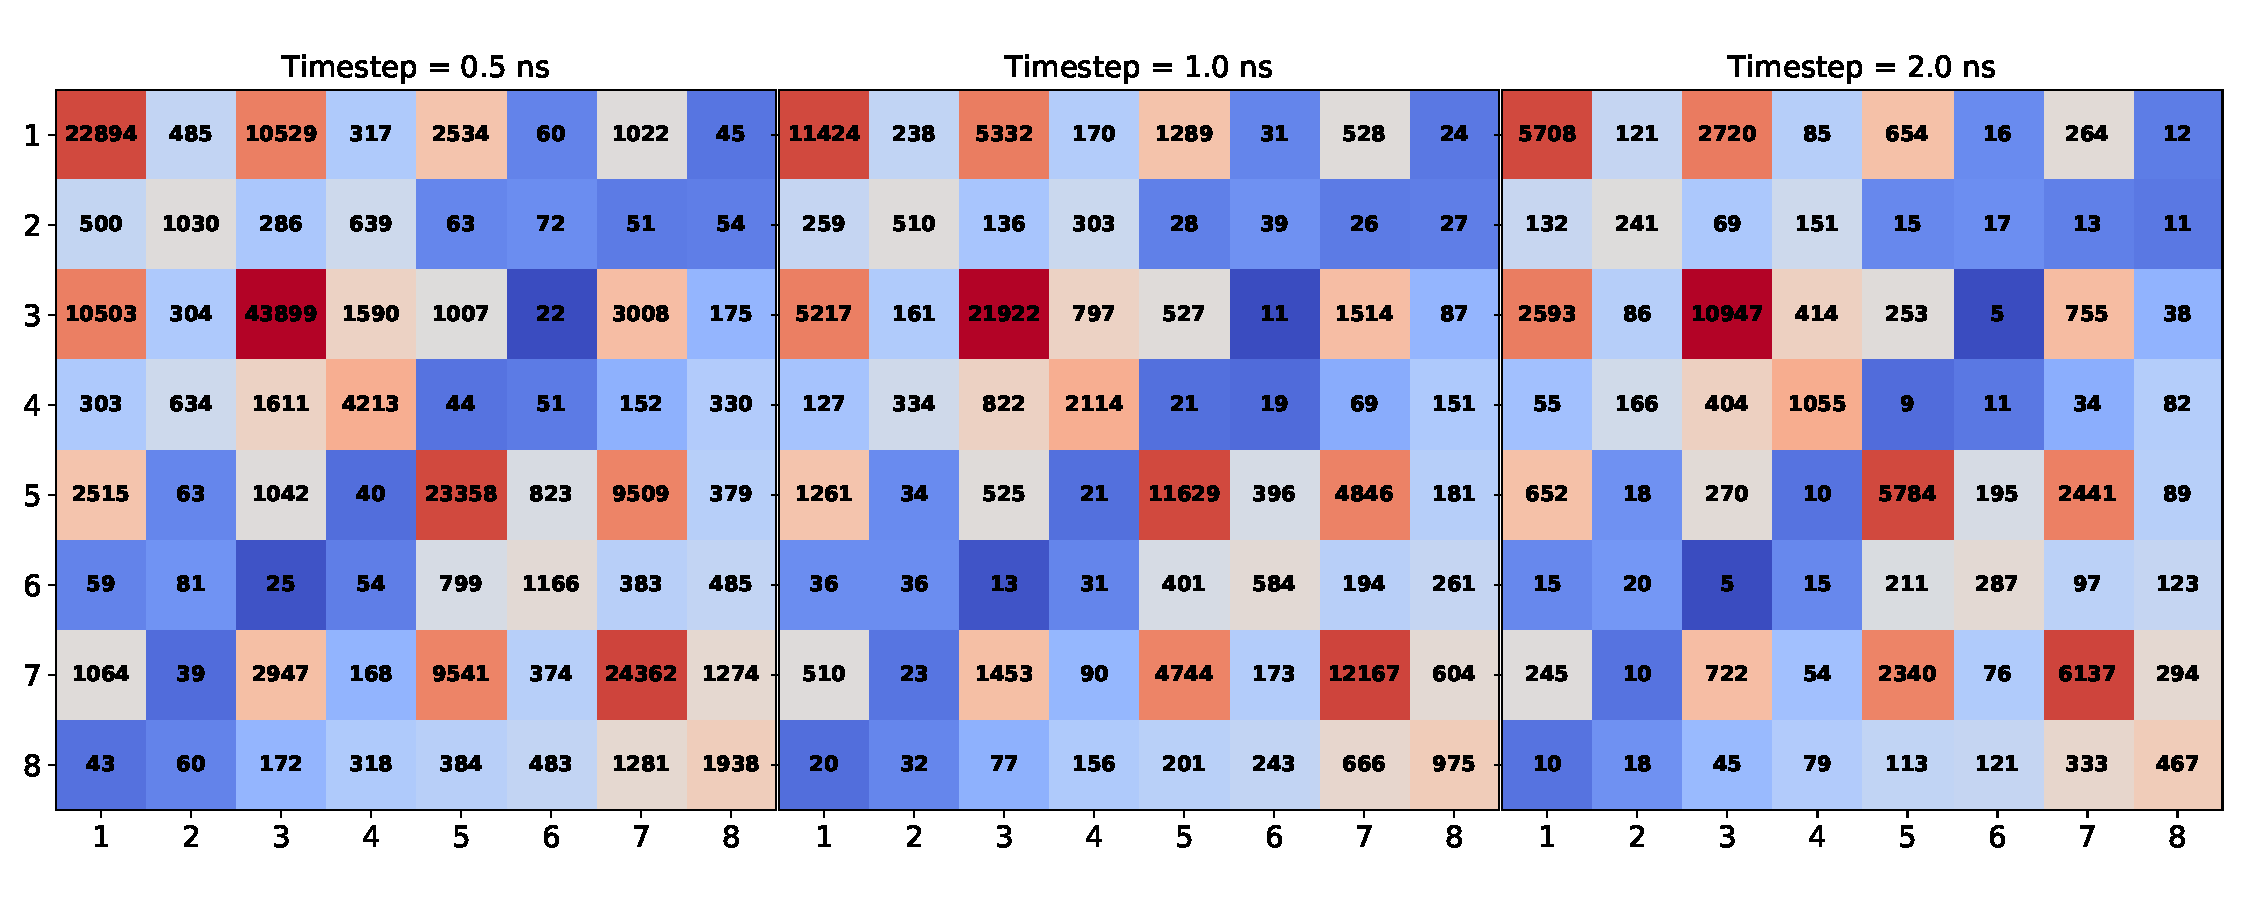
\includegraphics[width=\textwidth]{URE_counts.pdf}
  \caption{Urea}\label{fig:URE_counts}
  \end{subfigure}
  \begin{subfigure}{\textwidth}
  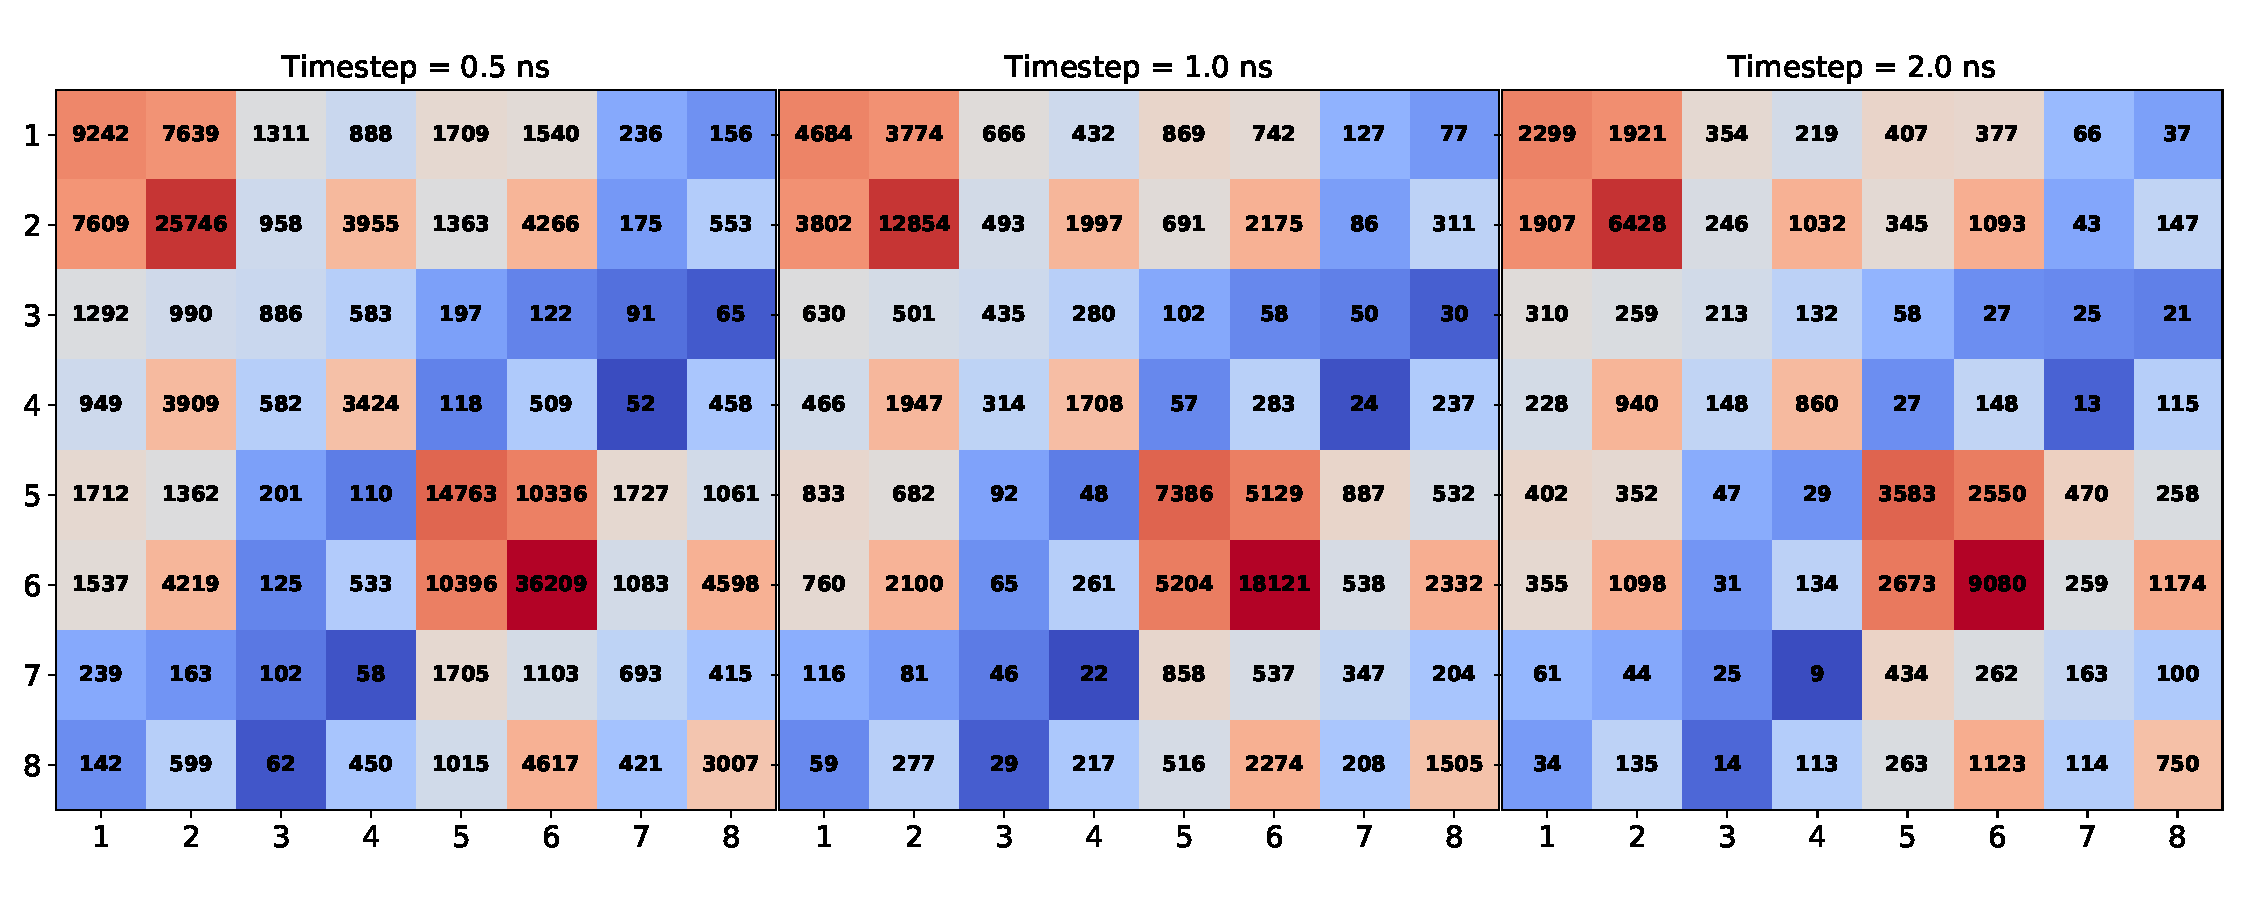
\includegraphics[width=\textwidth]{GCL_counts.pdf}
  \caption{Ethylene Glycol}\label{fig:GCL_counts}
  \end{subfigure}
  \caption{The number of transitions from state $i$ to $j$ and $j$ to $i$ are very close
  indicating that our process obeys detailed balance. Detailed balance is conserved for 
  different sized time steps.}\label{fig:counts}
  %MRS: would this be clearer to see if you plotted i-j/i+j for a relative error to see how different it is from symmetric jumps? 
  \end{figure}
  
  \begin{figure}
  \centering
  \begin{subfigure}{\textwidth}
  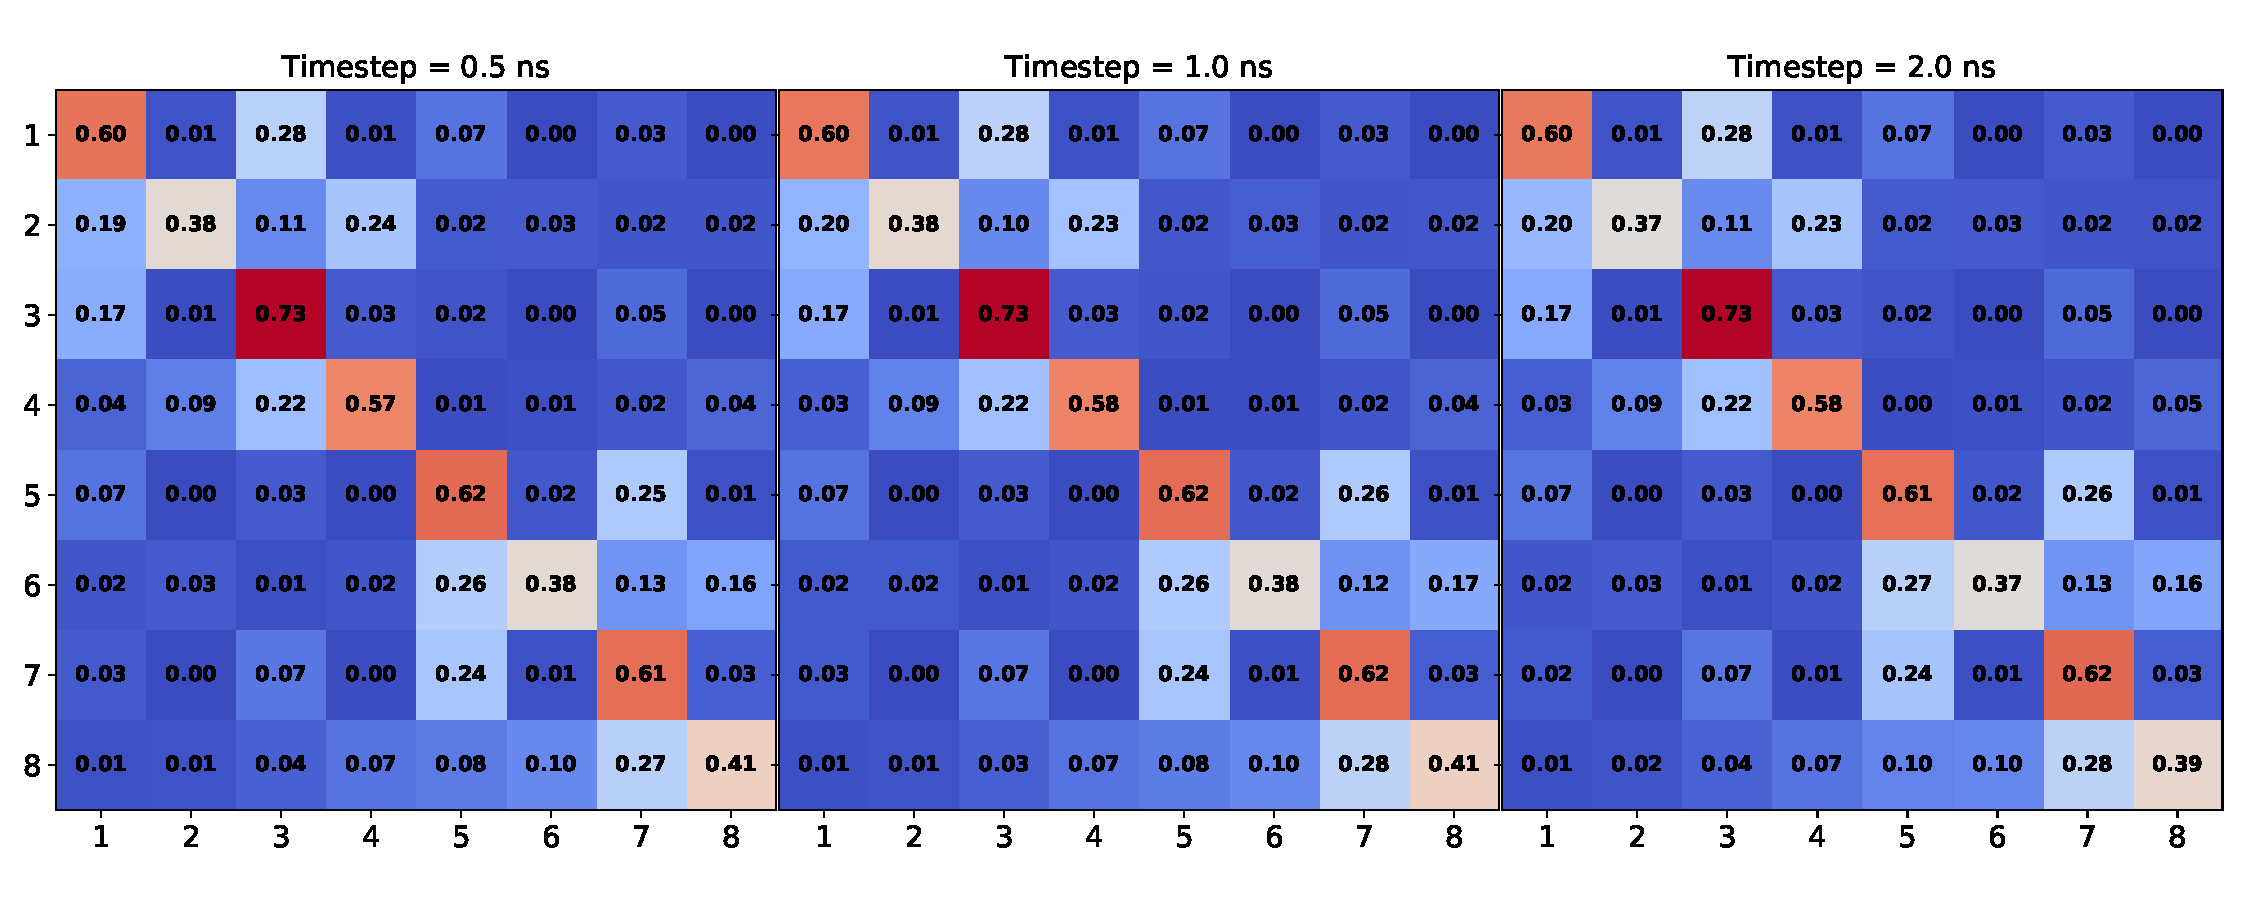
\includegraphics[width=\textwidth]{URE_transitions.pdf}
  \caption{Urea}\label{fig:URE_transitions}
  \end{subfigure}
  \begin{subfigure}{\textwidth}
  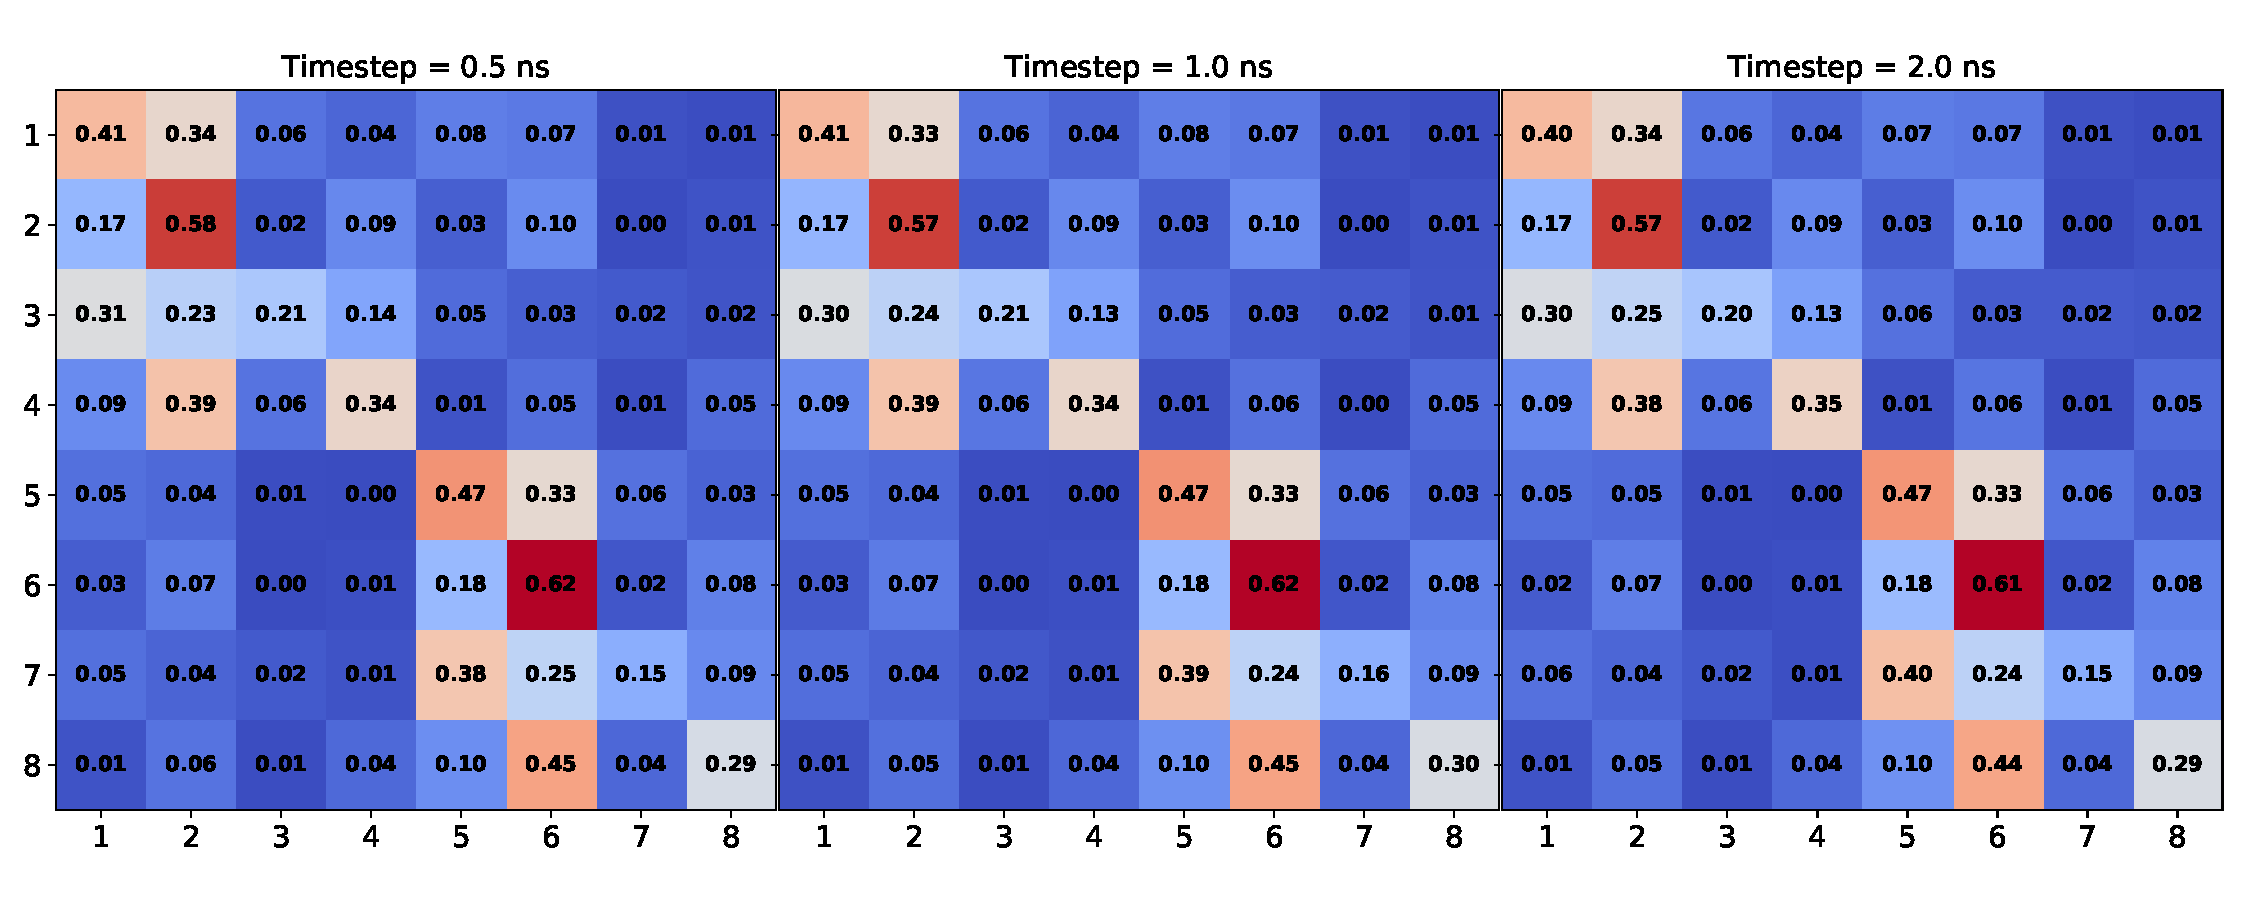
\includegraphics[width=\textwidth]{GCL_transitions.pdf}
  \caption{Ethylene Glycol}\label{fig:GCL_transitions}
  \end{subfigure}
  \caption{As the timestep between observations increases, the probability
  transition matrix does not change significantly.}\label{fig:transitions}
  \end{figure}
  
  \newpage  
  
  \section{Derivation of Passage Time Distributions}\label{section:fpt_derivation}
  
  To derive an analytical equation for the mean first passage time 
  (Equation~\ref{M-eqn:passage_times} of the main text), first consider an 
  initial pulse spreading out over time with a fixed mean. We can solve for the 
  time-dependent probability density of particle positions, $p$, by solving the one
  dimensional diffusion equation:
  \begin{equation}
  \frac{\partial p}{\partial t} = D \frac{\partial^2 p}{\partial z^2}
  \end{equation}
  The appropriate initial and boundary conditions are:
  $$BC1: t > 0, z = \infty, p = 0$$
  $$BC2: t > 0, z = 0, \frac{\partial p}{\partial z} = 0$$
  $$IC: t = 0, c = \delta(z)$$ % M\delta(z)
  %where $M$ is the total number of particles in the system. 
  It has been shown 
  elsewhere that the solution to this equation is:~\cite{cussler_diffusion:_2009}
  \begin{equation}
  p(z, t) = \frac{1}{\sqrt{4 \pi D t}}\exp\bigg(\frac{-z^2}{4Dt}\bigg)
  \end{equation}
  We can make the substitution $z = z - vt$, where $v$ represents a constant average
  velocity, in order to linearly shift the mean as a function of time:
  \begin{equation}
  p(z, t) = \frac{1}{\sqrt{4 \pi D t}}\exp\bigg(\frac{-(z - vt)^2}{4Dt}\bigg)
  \end{equation}
  One can track the fraction of particles, $F$, that have crossed the pore 
  boundary by integrating:
  \begin{equation}
  F(t) = \int_L^\infty p~dz = \mathrm{erfc}\bigg(\frac{L - vt}{2\sqrt{D t}}\bigg)
  \end{equation}
  where $L$ is the pore length. This represents the cumulative first passage 
  time distribution so we take its derivative in order to arrive at the first
  passage time distribution:
  \begin{equation}
  P(t) = -\frac{1}{\sqrt{\pi}}e^{-(L - vt)^2 / (4Dt)}\bigg(-\frac{D(L - vt)}{4(Dt)^{3/2}} - \frac{v}{2\sqrt{Dt}}\bigg)
  \label{eqn:passage_times}
  \end{equation} 
  where the only free parameters for fitting are $v$ and $D$. We calculated the
  expected value of Equation~\ref{eqn:passage_times} in order to get the MFPT. Specifically,
  we used the python package \texttt{scipy.integrate.quad} to numerically integrate:
  \begin{equation}
  E[t] = \int_0^\infty tP(t) dt
  \end{equation}
  
  \newpage
  
  \section{Solute hopping and trapping behavior}\label{section:sfbm_other_solutes}
  
  Analogous to Figure~\ref{M-fig:anticorrelated_hops} of the main text,
  Figure~\ref{fig:anticorrelated_hops} demonstrates that all solutes exhibit the
  same kind of anti-correlated hopping and trapping behavior.
  
  \begin{figure}[h]
  \centering
  % /figures/distributions_sfbm.py
  \begin{subfigure}{0.3\textwidth}
  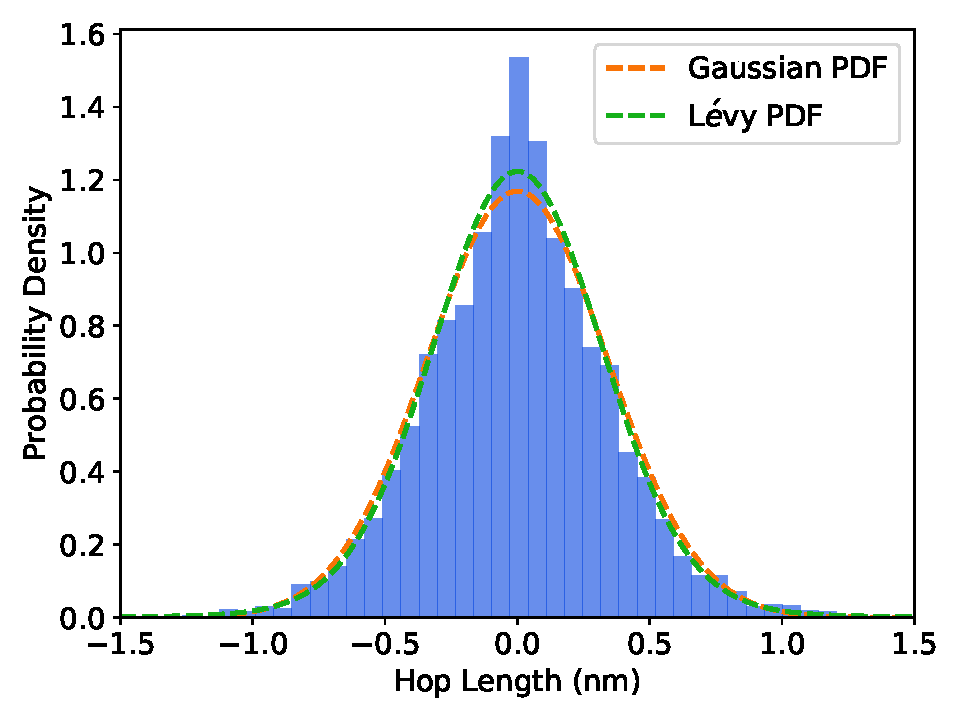
\includegraphics[width=\textwidth]{gaussian_levy_comparison_anomalous_GCL.pdf}
  \caption{}\label{fig:GCL_hop_distribution_comparison}
  \end{subfigure}
  \begin{subfigure}{0.3\textwidth}
  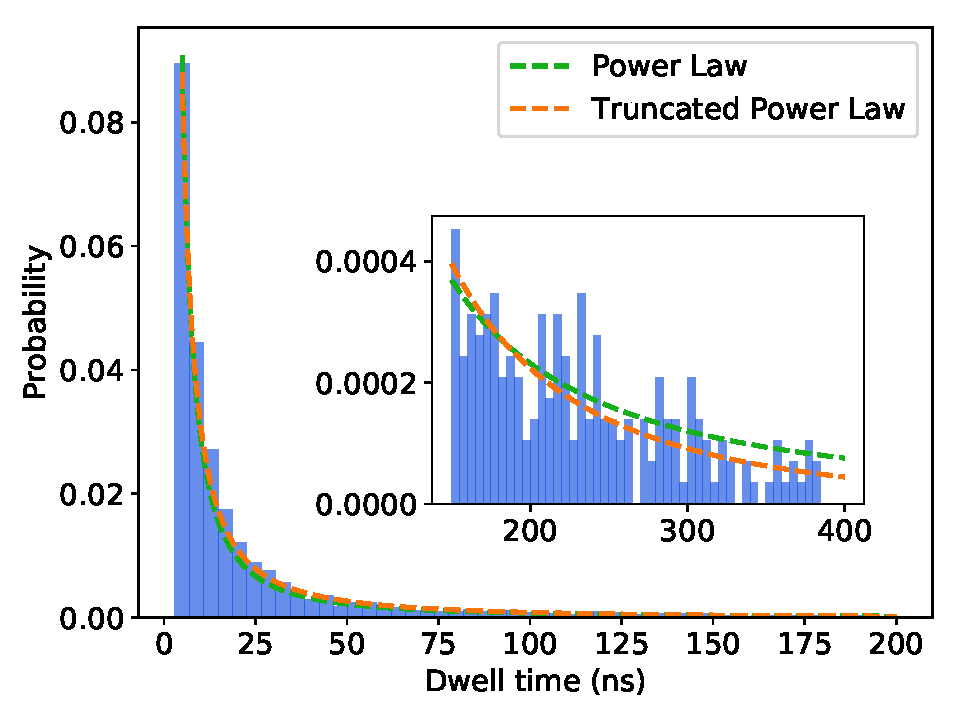
\includegraphics[width=\textwidth]{GCL_powerlaw.pdf}
  \caption{}\label{fig:GCL_powerlaw}
  \end{subfigure}
  \begin{subfigure}{0.3\textwidth}
  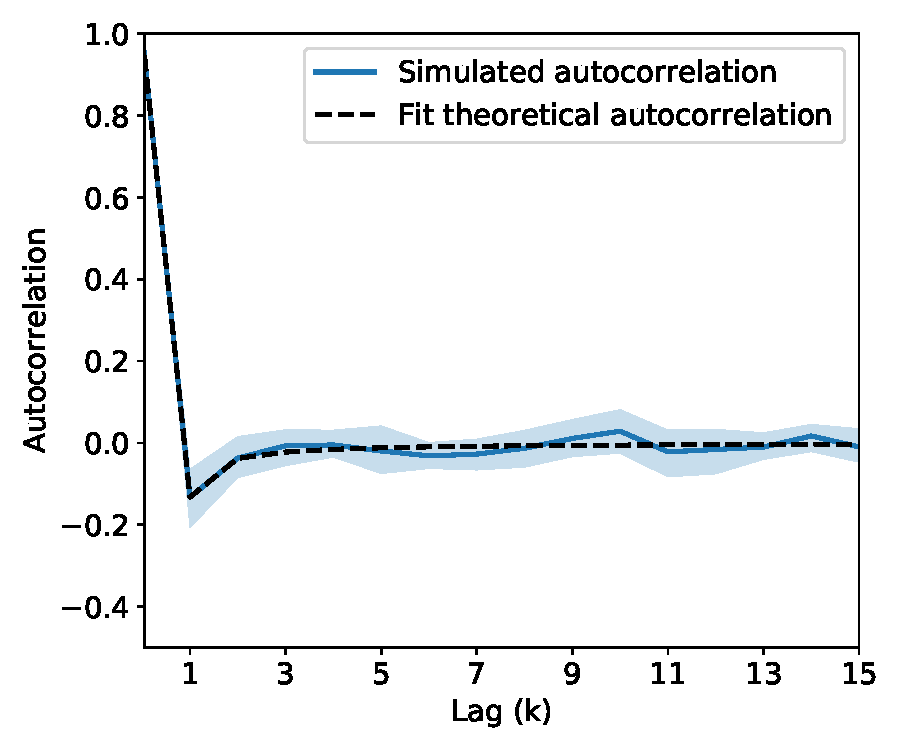
\includegraphics[width=\textwidth]{GCL_hop_acf.pdf}
  \caption{}\label{fig:GCL_hop_acf}
  \end{subfigure}
  \begin{subfigure}{0.3\textwidth}
  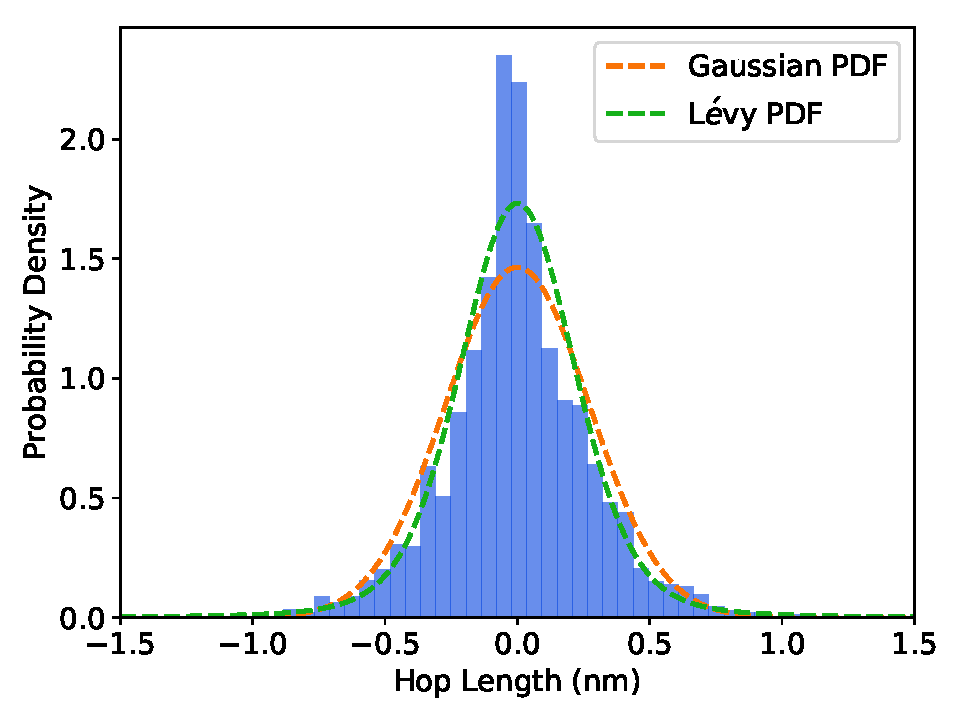
\includegraphics[width=\textwidth]{gaussian_levy_comparison_anomalous_ACH.pdf}
  \caption{}\label{fig:ACH_hop_distribution_comparison}
  \end{subfigure}
  \begin{subfigure}{0.3\textwidth}
  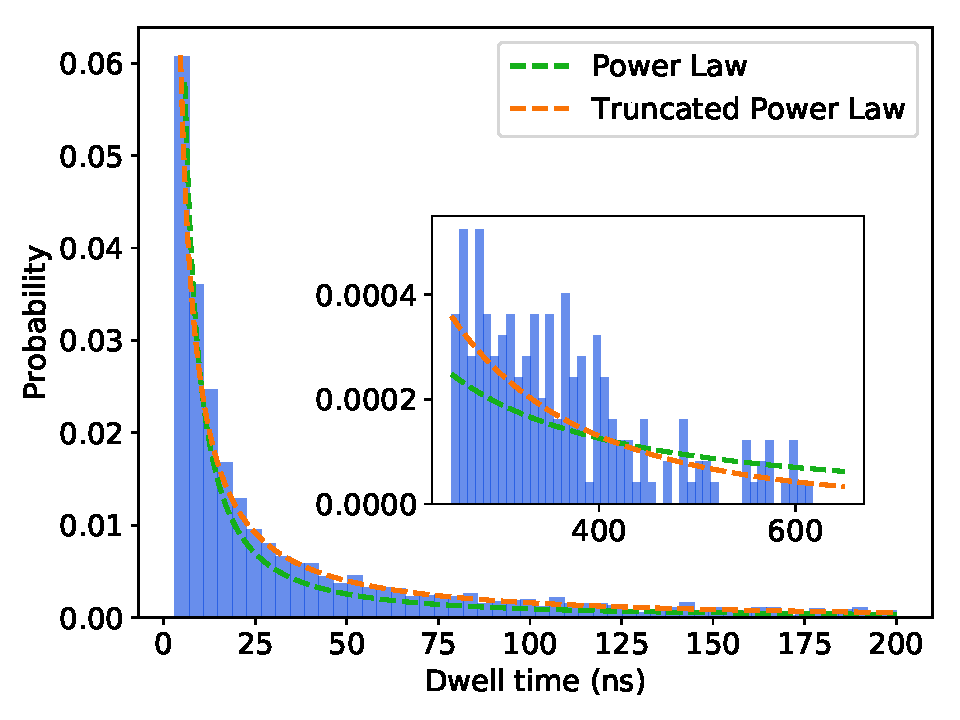
\includegraphics[width=\textwidth]{ACH_powerlaw.pdf}
  \caption{}\label{fig:ACH_powerlaw}
  \end{subfigure}
  \begin{subfigure}{0.3\textwidth}
  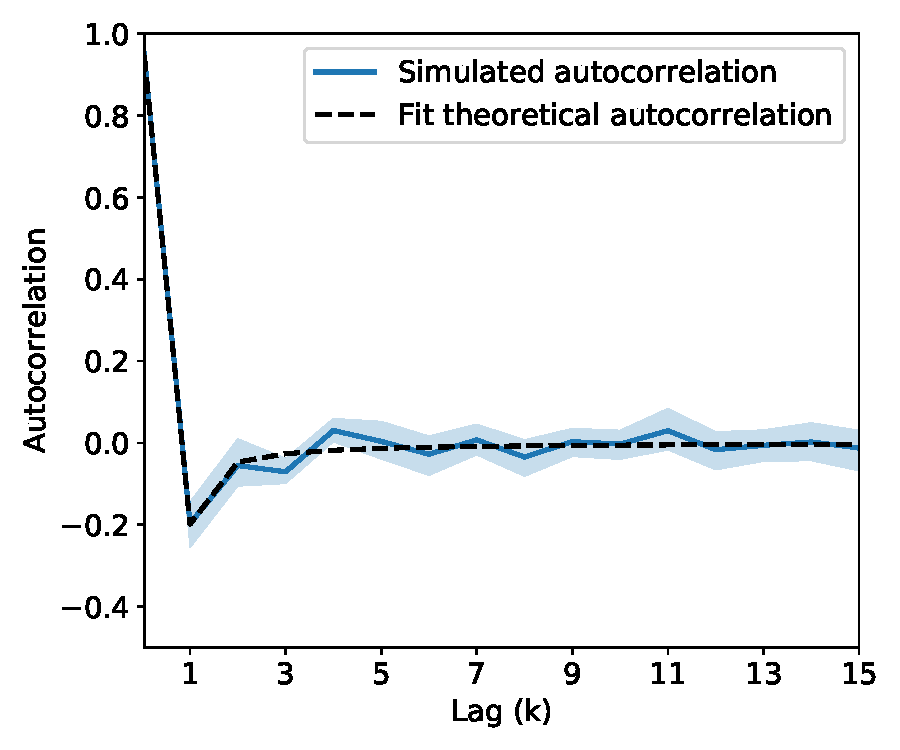
\includegraphics[width=\textwidth]{ACH_hop_acf.pdf}
  \caption{}\label{fig:ACH_hop_acf}
  \end{subfigure}
  \begin{subfigure}{0.3\textwidth}
  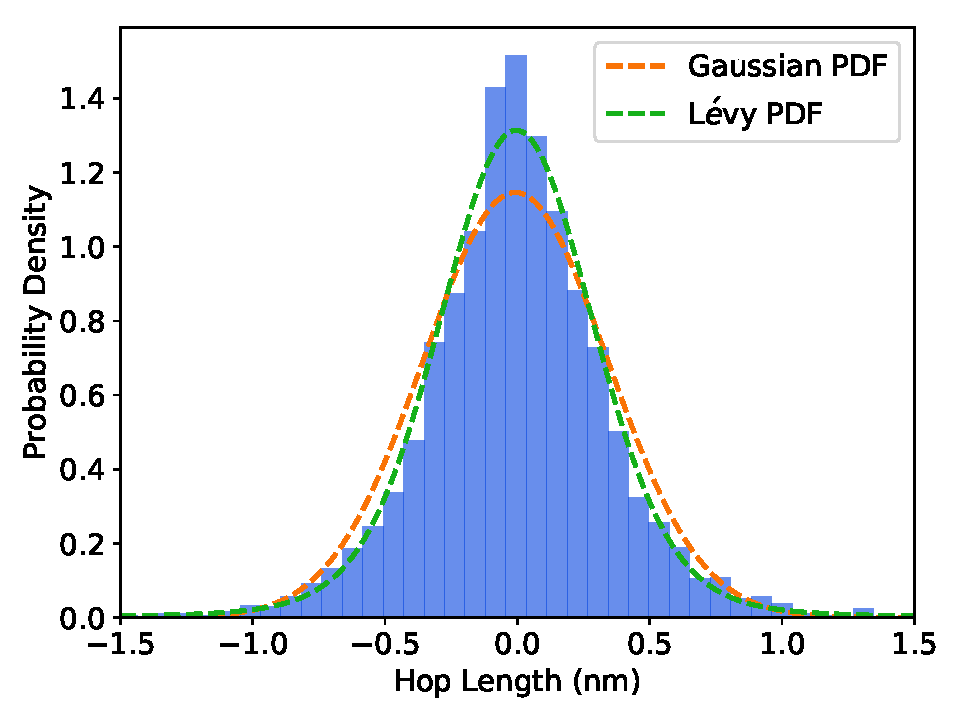
\includegraphics[width=\textwidth]{gaussian_levy_comparison_anomalous_MET.pdf}
  \caption{}\label{fig:MET_hop_distribution_comparison}
  \end{subfigure}
  \begin{subfigure}{0.3\textwidth}
  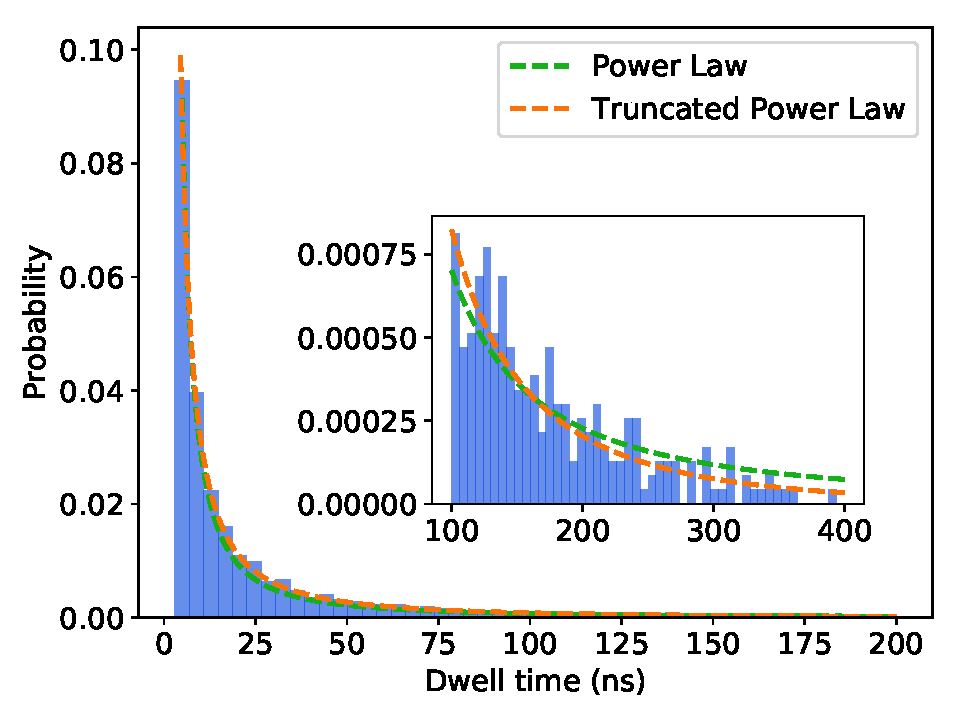
\includegraphics[width=\textwidth]{MET_powerlaw.pdf}
  \caption{}\label{fig:MET_powerlaw}
  \end{subfigure}
  \begin{subfigure}{0.3\textwidth}
  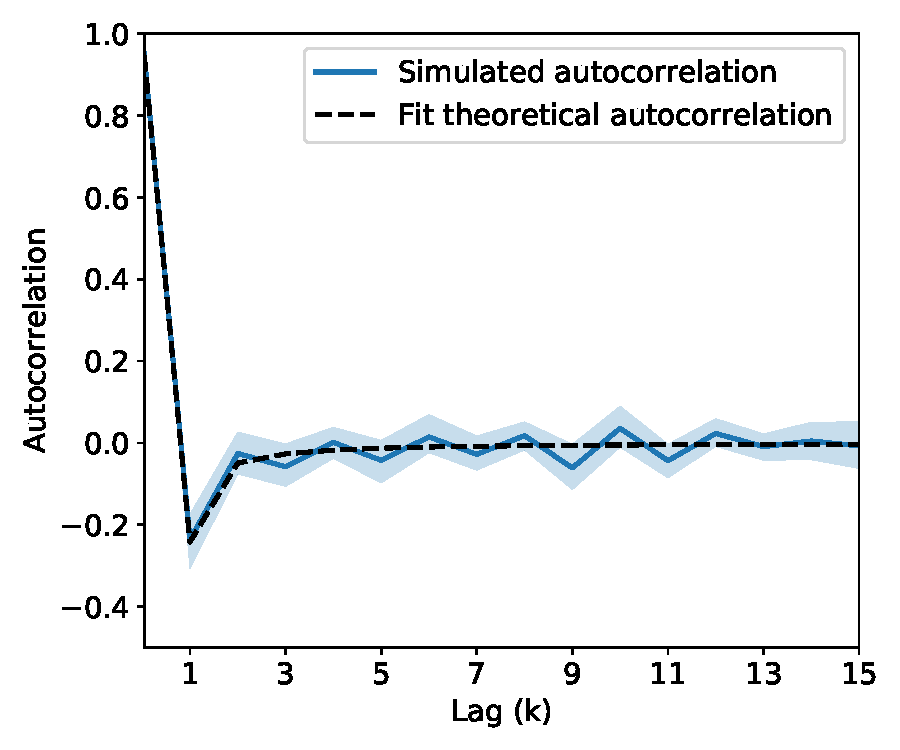
\includegraphics[width=\textwidth]{MET_hop_acf.pdf}
  \caption{}\label{fig:MET_hop_acf}
  \end{subfigure}
  \caption{Hop length distributions, dwell time distributions and hop autocorrelation functions
  respectively for ethylene glycol (a-c), acetic acid (d-f) and methanol (g-i).
  See Section~\ref{M-section:AD_parameterization} of the main text for a more detailed discussion.
  }\label{fig:anticorrelated_hops}
  \end{figure}
  
  \newpage
  
  \section{AD model MSD Predictions with Pure Power Law Dwell Times}\label{section:pure_power_law}
  
  When we use a pure power law distribution to parameterize the dwell time 
  distributions of the 1 and 2 mode AD models, the MD MSDs are severely 
  under-predicted because we are incorporating dwell times on the order of 
  the simulation length into simulated trajectories 
  (see Figure~\ref{fig:anomalous_msds_bothmode}). The parameters of the pure power law 
   distribution are included in Figure~\ref{fig:pure_power_law_params}. 
  
  \begin{figure}[h]
  \centering
  \begin{subfigure}{0.45\textwidth}
  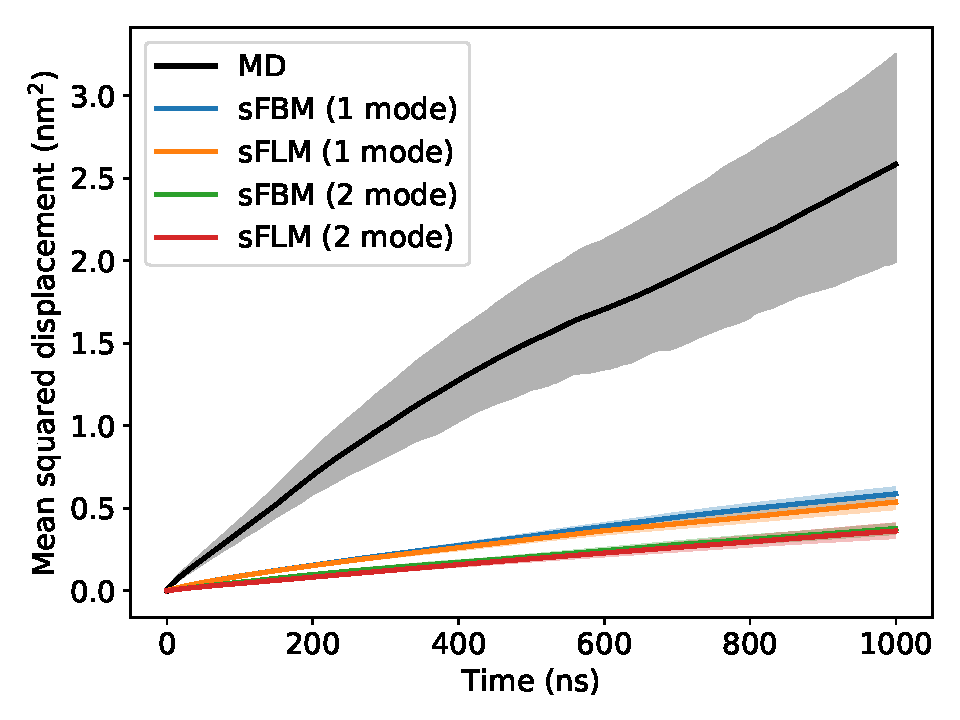
\includegraphics[width=\textwidth]{bothmode_msd_comparison_URE.pdf}
  \caption{Urea}\label{fig:bothmode_msd_comparison_URE}
  \end{subfigure}
  \begin{subfigure}{0.45\textwidth}
  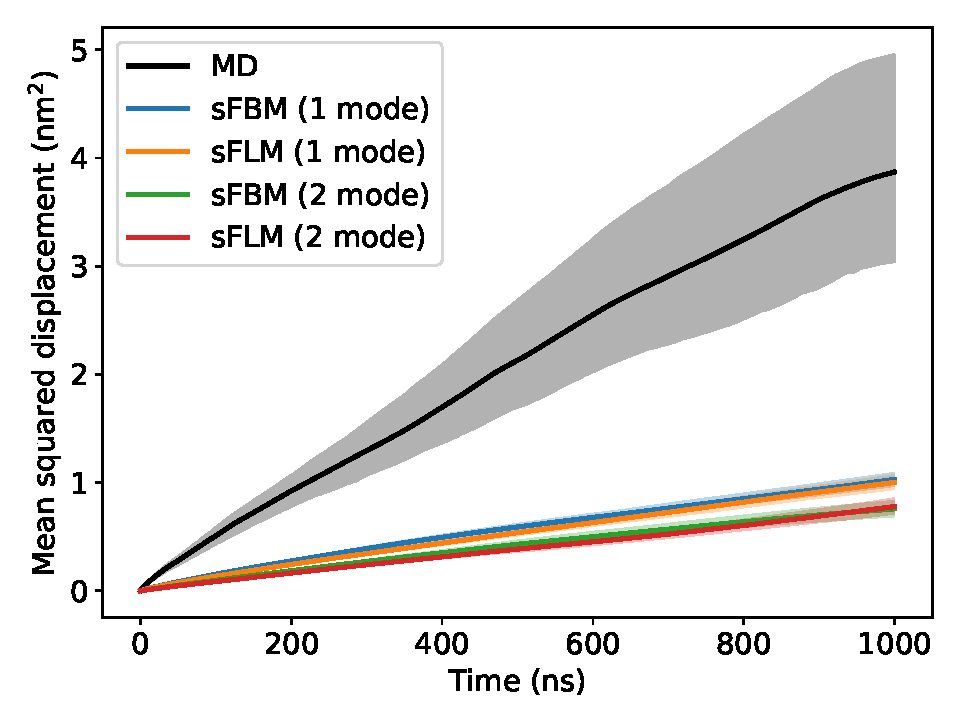
\includegraphics[width=\textwidth]{bothmode_msd_comparison_GCL.pdf}
  \caption{Ethylene Glycol}\label{bothmode_msd_comparison_GCL}
  \end{subfigure}
  \begin{subfigure}{0.45\textwidth}
  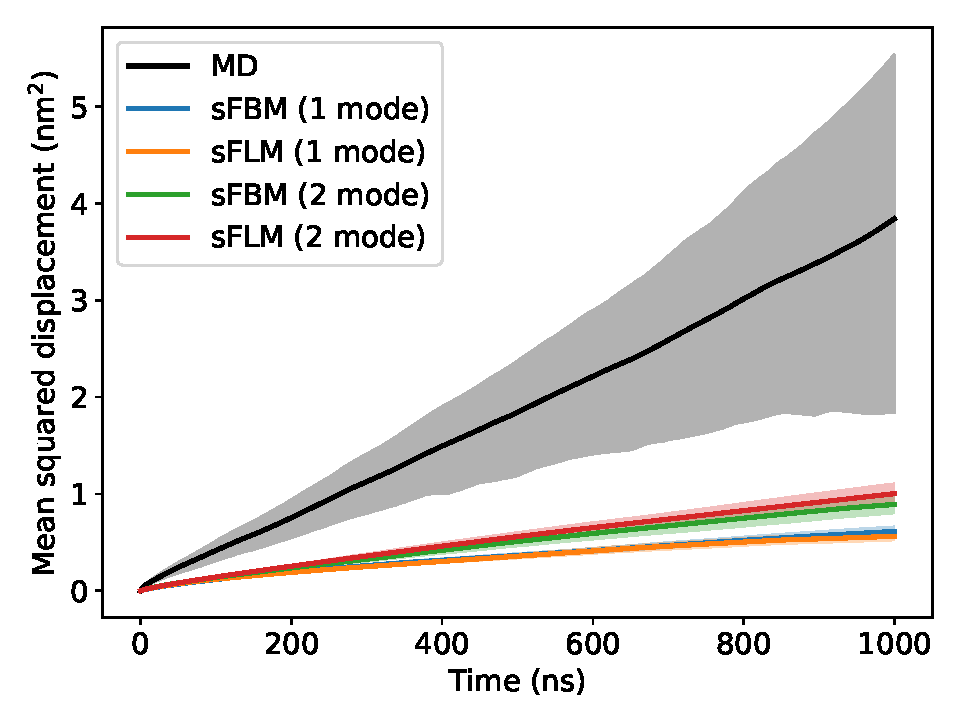
\includegraphics[width=\textwidth]{bothmode_msd_comparison_MET.pdf}
  \caption{Methanol}\label{fig:bothmode_msd_comparison_MET}
  \end{subfigure}
  \begin{subfigure}{0.45\textwidth}
  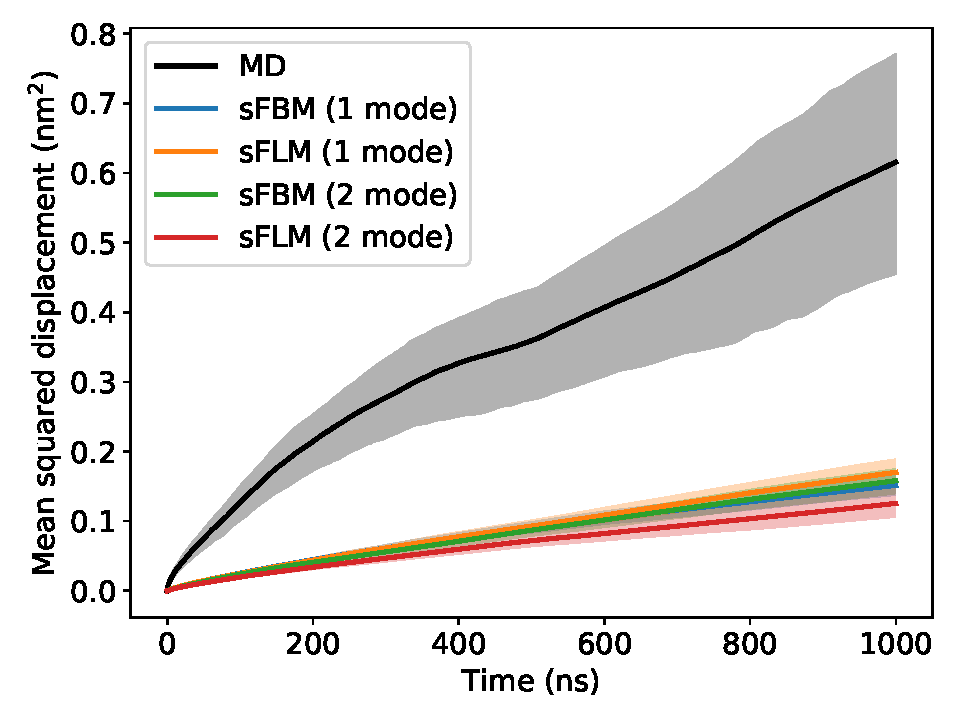
\includegraphics[width=\textwidth]{bothmode_msd_comparison_ACH.pdf}
  \caption{Acetic Acid}\label{fig:bothmode_msd_comparison_ACH}
  \end{subfigure}
  \caption{When we do not apply an exponential cut-off to the power law
  distribution of dwell times,  MSDs are consistently under-predicted by the
  AD model.
  }\label{fig:anomalous_msds_bothmode}
  \end{figure}
  
  \begin{figure}
  \centering
  \begin{subfigure}{0.45\textwidth}
  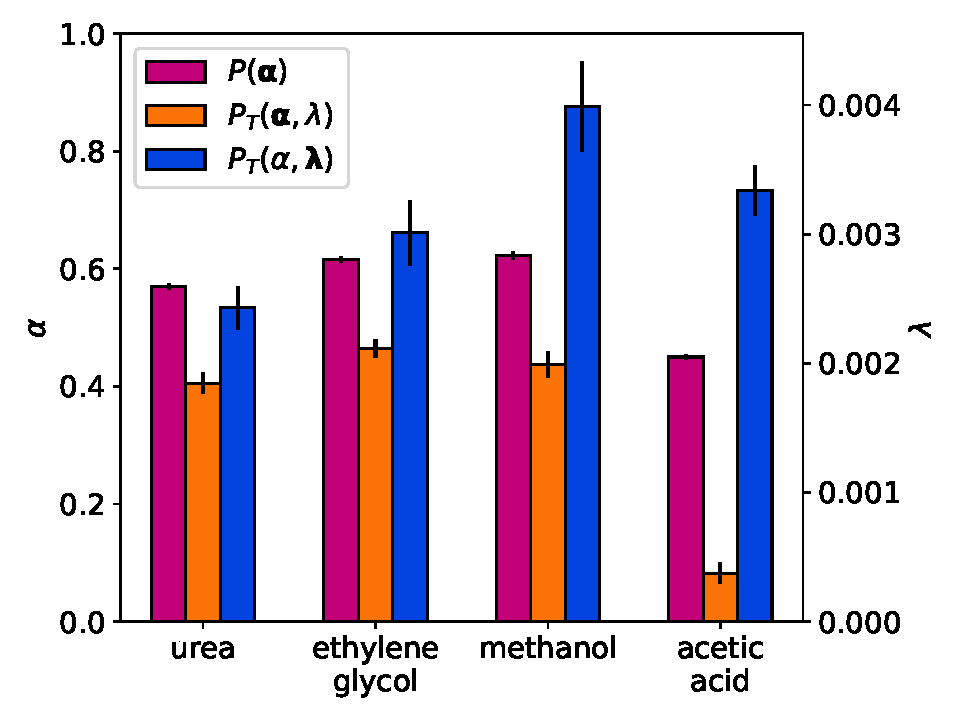
\includegraphics[width=\textwidth]{1mode_AD_dwells.pdf}
  \caption{}\label{fig:1mode_AD_dwells}
  \end{subfigure}
  \begin{subfigure}{0.45\textwidth}
  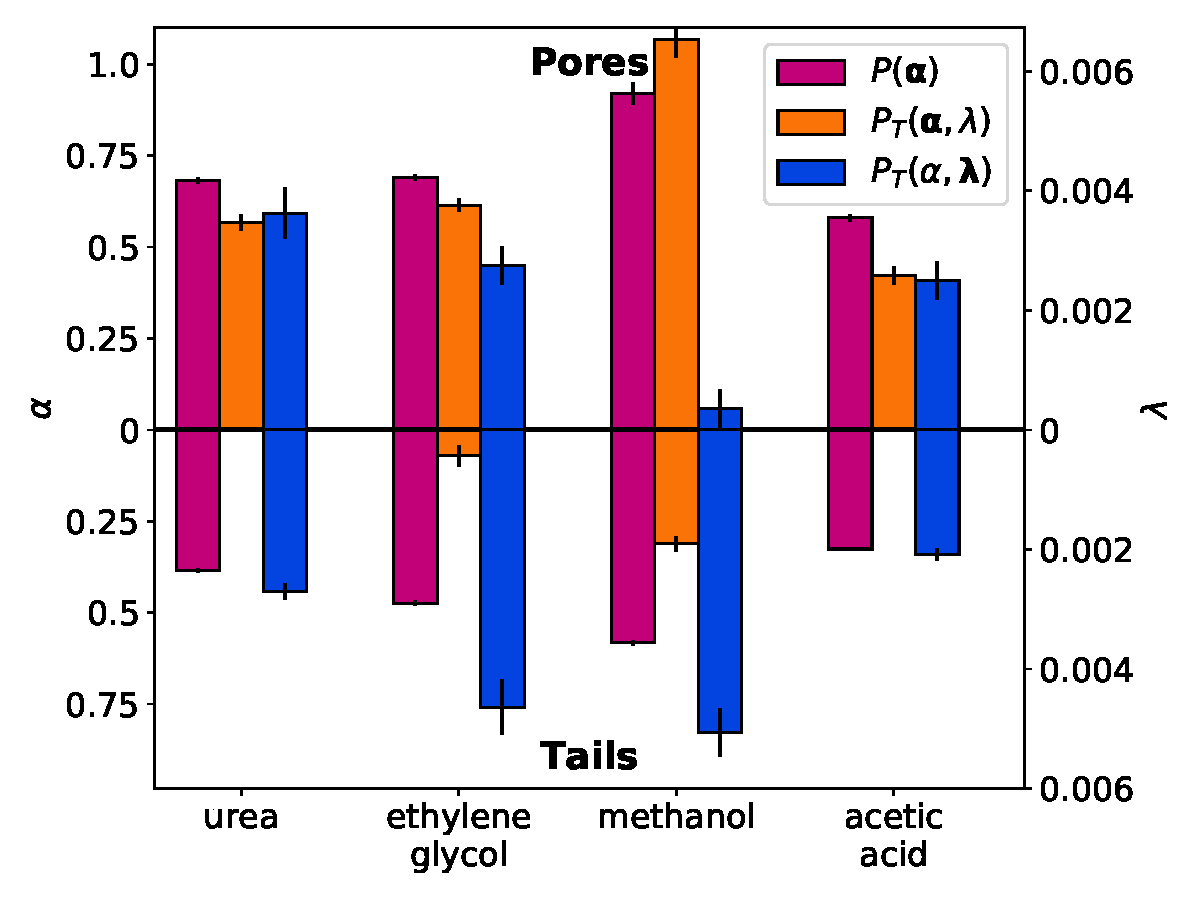
\includegraphics[width=\textwidth]{2mode_AD_dwells.pdf}
  \caption{}\label{fig:2mode_AD_dwells}
  \end{subfigure}
  \caption{We can parameterize the dwell time distribution in two ways: as a pure
  power law (P($\alpha$)) and as a power law with an exponential cut-off (P($\alpha$, $\lambda$)).
  Pure power laws have an infinite variance which allows extremely long dwell
  times to be sampled (see Figure~\ref{fig:anomalous_msds_bothmode}.
  }\label{fig:pure_power_law_params}
  \end{figure} 
  
  \newpage
  
  \section{Stationarity of Solute Trajectories}\label{section:msd_comparison}
  
  We evaluated the predictive capabilities of the AD modeling approach by training
  the model parameters on the first half of the equilibrated MD trajectory data and
  then comparing the MSD calculated from AD model realizations to the MSD calculated
  from the second half of the equilibrated MD trajectory data. This metric is
  only meaningful if the ensemble of solute trajectories is stationary. In 
  Figure~\ref{fig:msd_comparison}, we show that urea and acetic acid show acceptable
  stationary behavior while methanol and ethylene glycol do not.
  
  We validated both the 1 and 2 mode AD models with urea and acetic acid, since their
  trajectories appear stationary. The MSDs resulting from 1000 realizations of the AD
  model are shown in Figure~\ref{fig:train_test}. We consider the model's prediction 
  to match well if the MSD lies within the 1$\sigma$ confidence intervals of the MD MSDs.
  We also look for qualitative agreement in the shape of the curves.
  
  The models are capable of reasonably predicting the MD MSD values of the second
  half of the solute trajectories based on parameters generated from the first half
  when the dwell time distributions are parameterized by a power law with an 
  exponential cut-off. At long timescales, the MSD of urea is under-predicted 
  for both the 1 and 2 mode models with the same true of acetic acid on short 
  timescales. Without truncation of the power law distribution, the MD 
  MSDs are underestimated in all cases because dwell times on the order of the
  MD simulation length are sampled and incorporated into the simulated anomalous
  diffusion trajectories. 
  
  \begin{figure}[h]
  \centering
  \begin{subfigure}{0.45\textwidth}
  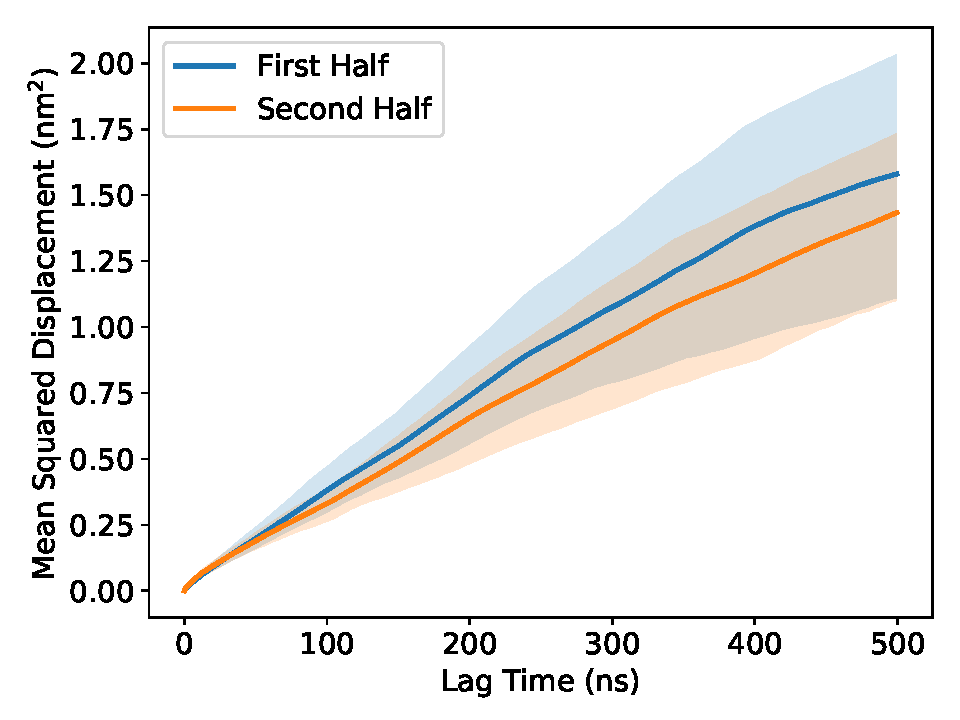
\includegraphics[width=\textwidth]{URE_MSD_halves.pdf}
  \caption{Urea}\label{fig:URE_MSD_halves}
  \end{subfigure}
  \begin{subfigure}{0.45\textwidth}
  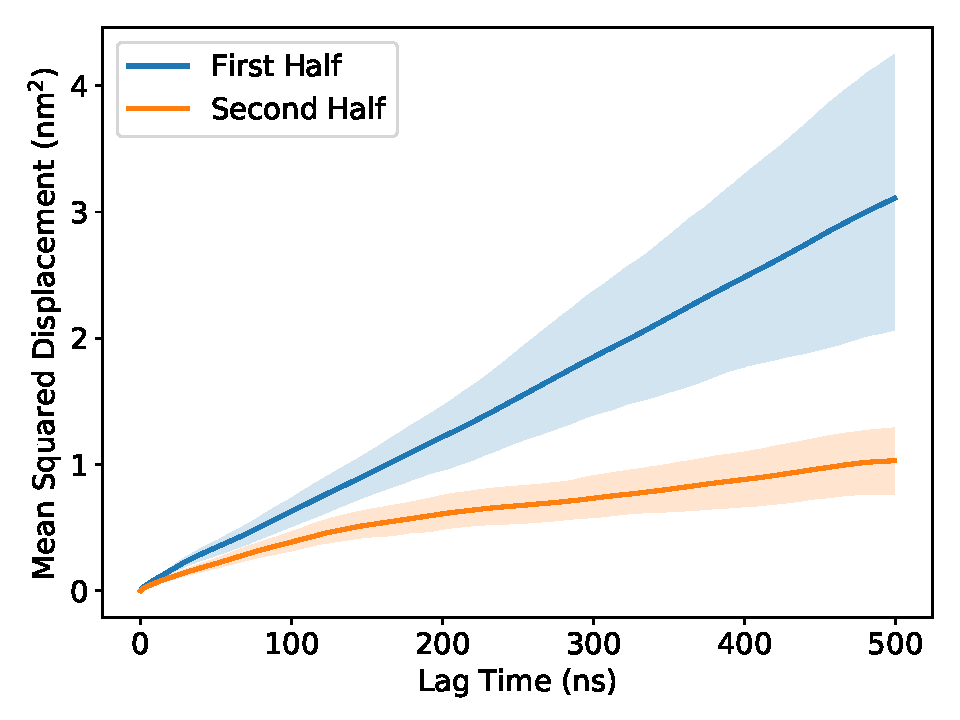
\includegraphics[width=\textwidth]{GCL_MSD_halves.pdf}
  \caption{Ethylene Glycol}\label{fig:GCL_MSD_halves}
  \end{subfigure}
  \begin{subfigure}{0.45\textwidth}
  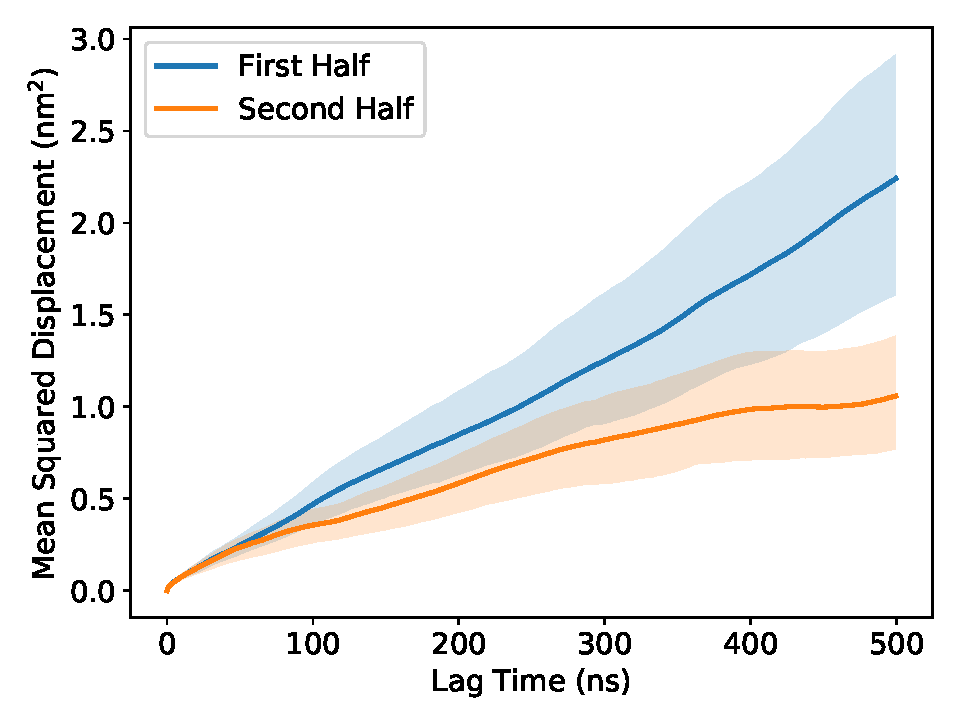
\includegraphics[width=\textwidth]{MET_MSD_halves.pdf}
  \caption{Methanol}\label{fig:MET_MSD_halves}
  \end{subfigure}
  \begin{subfigure}{0.45\textwidth}
  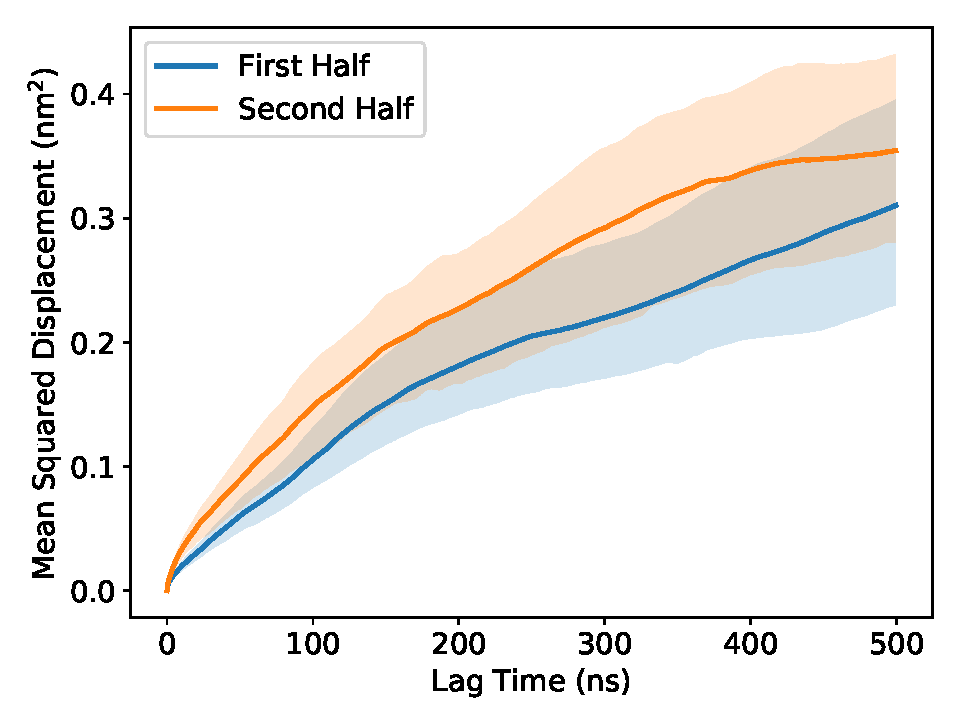
\includegraphics[width=\textwidth]{ACH_MSD_halves.pdf}
  \caption{Acetic Acid}\label{fig:ACH_MSD_halves}
  \end{subfigure}
  \caption{The ensemble of solute trajectories may be stationary if the MSD
  calculated from different portions of the trajectory are the same. Here we
  plot the MSD calculated up to a 500 ns time lag of the first and second
  halves of the equilibrated solute trajectories. Urea and acetic acid have
  similar MSDs, providing evidence of stationarity, while the MSDs of 
  ethylene glycol and methanol are different suggesting that they are not.}\label{fig:msd_comparison}
  \end{figure}

  \newpage
  
  \begin{figure}
  \centering
  \begin{subfigure}{0.45\textwidth}
  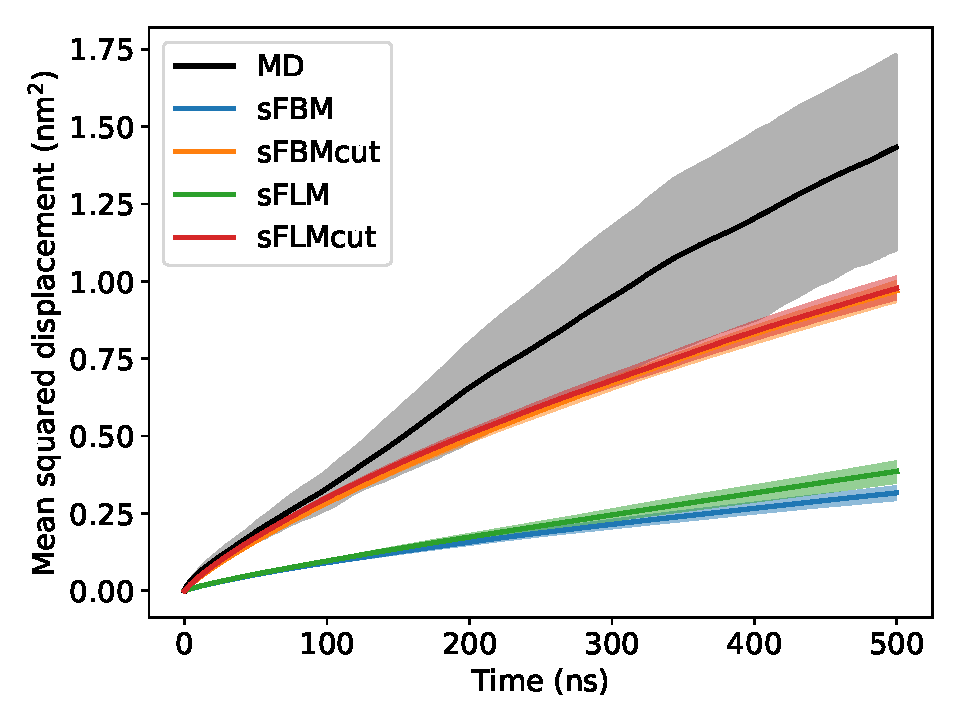
\includegraphics[width=\textwidth]{1mode_msd_comparison_URE_train_front.pdf}
  \caption{Urea (1 mode)}\label{fig:1mode_msd_comparison_URE_train_front}
  \end{subfigure}
  \begin{subfigure}{0.45\textwidth}
  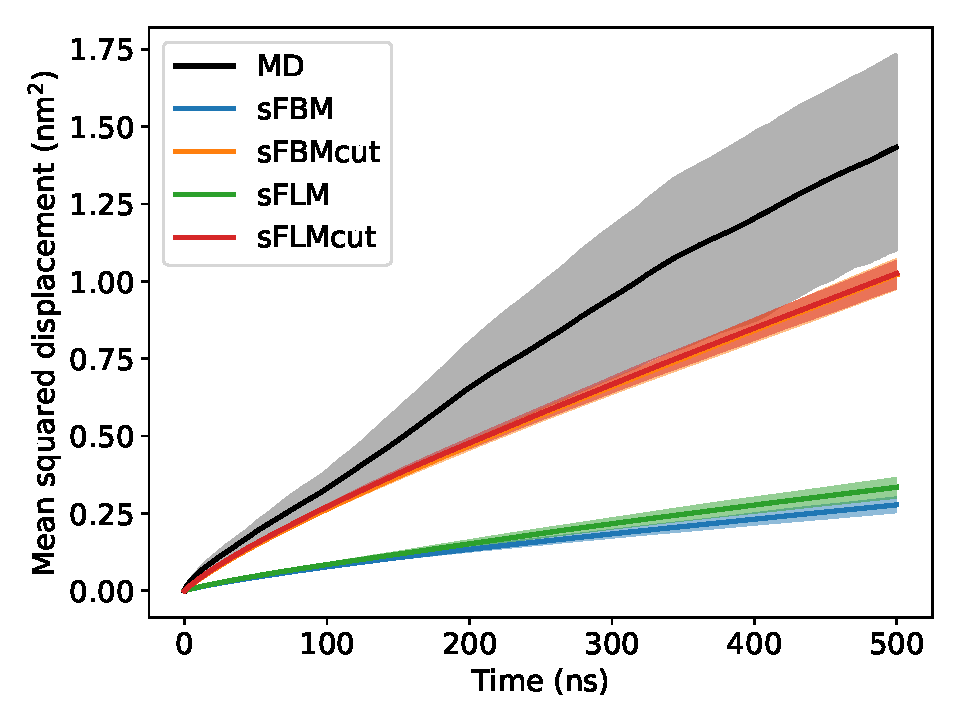
\includegraphics[width=\textwidth]{2mode_msd_comparison_URE_train_front.pdf}
  \caption{Urea (2 modes)}\label{fig:2mode_msd_comparison_URE_train_front}
  \end{subfigure}
  \begin{subfigure}{0.45\textwidth}
  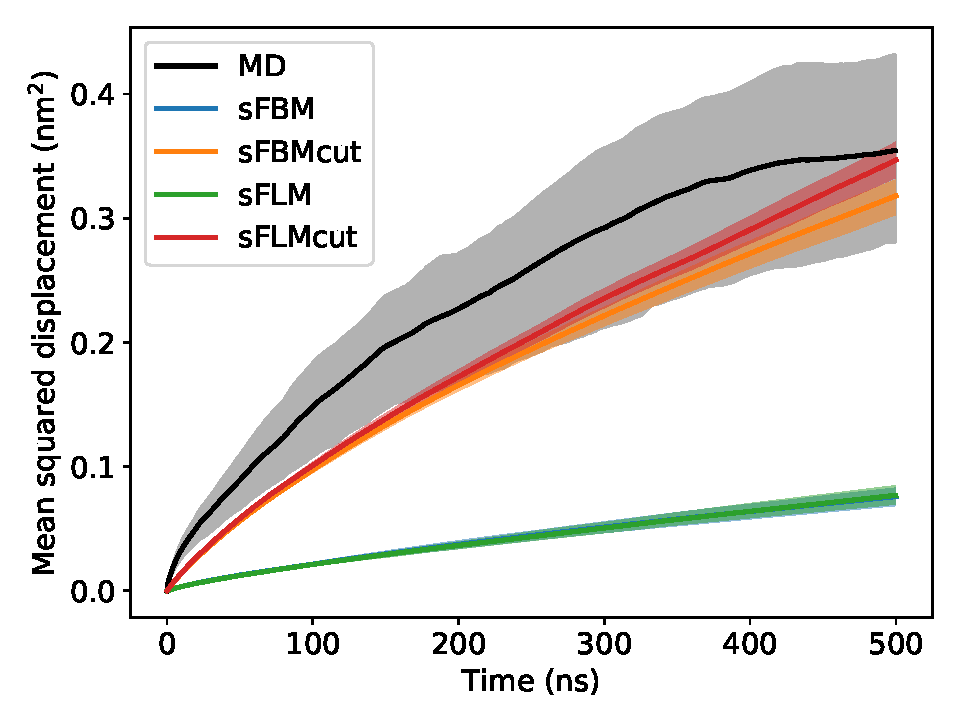
\includegraphics[width=\textwidth]{1mode_msd_comparison_ACH_train_front.pdf}
  \caption{Acetic acid (1 mode)}\label{fig:1mode_msd_comparison_ACH_train_front}
  \end{subfigure}
  \begin{subfigure}{0.45\textwidth}
  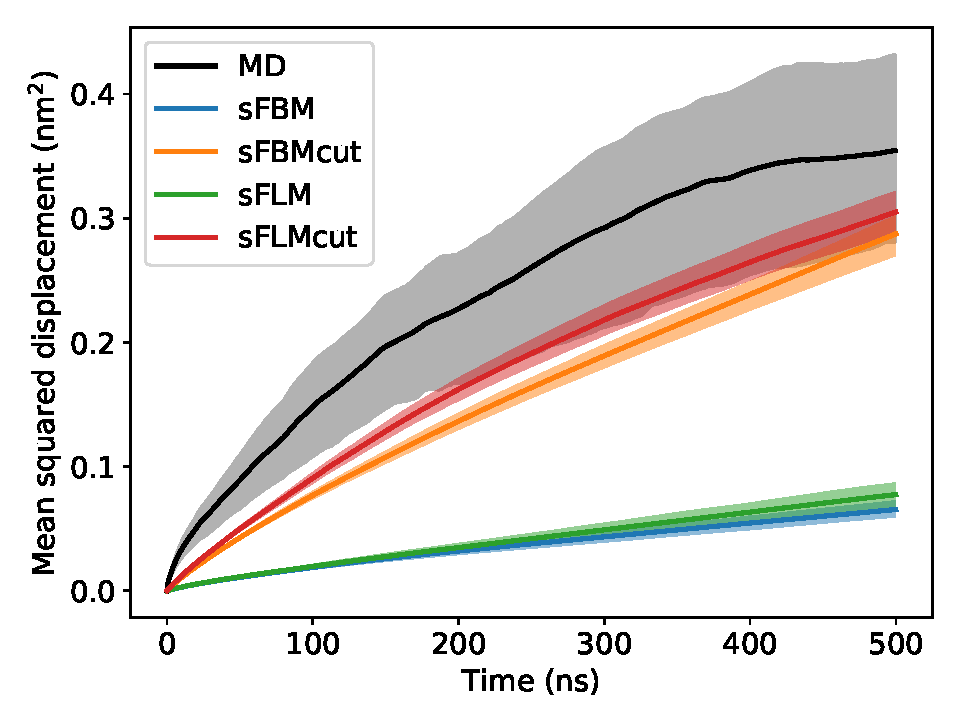
\includegraphics[width=\textwidth]{2mode_msd_comparison_ACH_train_front.pdf}
  \caption{Acetic acid (2 modes)}\label{fig:2mode_msd_comparison_ACH_train_front}
  \end{subfigure} 
  \caption{In most cases, when using power laws with exponential cut-offs 
  (sFBMcut and sFLMcut), the MSD curves predicted by the AD model trained on 
  the first half of the equilibrated data lie within the 1$\sigma$ confidence
  intervals of the MD MSD curves generated from the second half of the equilibrated
  solute data. The models which use pure power laws systematically under-predict
  the MD MSD curves. Over- and under-estimated curvature of the of urea and acetic acid's 
  MSD curves respectively causes the magnitude of urea's predicted MSDs to be 
  under-predicted at long timescales and those of acetic acid to be under-predicted
  at short timescales. Note that the sFBMcut and sFLMcut models are the same as 
  those in the main text.}\label{fig:train_test}
  \end{figure}
  
  %Considering the longest observed dwell time among all
  %solutes was 1.3 $\mu$s by ethylene glycol, we believe truncation is well-justified.
  %Although in most cases, the predicted MSD curves overlap the 1-$\sigma$ confidence
  %intervals of the MD MSD curves, they appear to lie systematically below the mean. 
  %It is not clear whether this is a consistent feature of the AD model since we 
  %only used 2 solutes for this analysis. 
  
%  We also observe that simulated AD trajectories which draw from a L\'evy stable 
%  distribution generally predict higher MSDs. The heavy tails of the distribution 
%  incorporate large jumps more frequently into the trajectories. 
  
%  From a qualitative perspective, the models only have moderate success at predicting
%  the shape of the MSD curves. Error in the MSD curvature can also help explain some of
%  the error in the predicted MSD magnitudes. The curves predicted for urea with both 1 
%  and 2 modes appear to have too much curvature, which causes it to under-predict the 
%  MSD at long timescales, while those of acetic acid lack curvature, leading the
%  AD model to under-predict the MSD at short timescales. 
  
  %MRS8: how much of this is already in the main text?  Try to limit analysis that appears in the main text.
%  The under-estimate of urea's MSD at long timescales is due to long timescale
%  positional anti-correlation which may not be present in the molecularly 
%  detailed simulations of the system. The 
%  persistent curvature of the predicted MSD curves is a direct consequence of 
%  the Hurst parameter. Without anti-correlation, the process would be 
%  a pure CTRW for which one would expect the time averaged MSD curves to become 
%  linear.~\cite{meroz_toolbox_2015} It may be true that on the $\mu$s time scale, 
%  positional correlation is lost which would manifest as a transition from a sub-linear
%  to linear MSD curve. A solution for more accurately modeling this behavior in  
%  the future may be to truncate the positional autocorrelation function.~\cite{molina-garcia_crossover_2018}
%  
%  The under-estimate of the curvature of acetic acid's predicted MSD suggests that,
%  in this case, the AD model over-estimates the Hurst parameter. This is not surprising
%  because the Hurst parameter is challenging to quantify, especially with a relatively 
%  small amount of data (see Section~\ref{M-method:sfbm} of the main text for further discussion of this 
%  challenge). A more accurate measurement of $H$ would fix the shape of the MSD curve,
%  but also lower the predicted MSD meaning we are either underestimating the width of
%  the hop length distribution, favoring longer dwell times, or both.
%  
%  This brief qualitative analysis suggests two shortcomings of the AD model. First, in
%  a real system, positional anti-correlation may dissipate after a sufficiently long 
%  time lag, dependent on the solute being studied. Second, it is difficult to reliably
%  parameterize the Hurst parameter which is important for accurately describing the 
%  curvature of the solute MSDs.
%  
%  This analysis also suggests that working with only half of the data we collected
%  ($\sim$ 2 $\mu$s post-equilibration) is not always sufficient for extracting reliable
%  parameter estimates. In most cases, the magnitude of the MSD predictions after a 
%  500 ns time lag are within or close to within error of the MD MSDs (for sFBMcut and
%  sFLMcut), but still appear to systematically under-predict the mean. We may be
%  operating on the border of the minimum amount of data required to accurately 
%  parameterize the AD model. Longer simulations and more independent trajectories may
%  be necessary. Therefore, in the next section we will work with parameters fit to the
%  full equilibrated portion of the solute trajectories, doubling the data.
  
%MRS6: My instinct is to only show the graphs of the full model, with validation graphs shown in the supporting.  We can talk about this. We do what the focus to be on what we can learn physically.  The discussion gets pretty repetitive.
  
%MRS6: be a bit clearer about how the MD MSD error bounds are calculated.  That becomes important for determining how accurate the modeling is. . 

%  However, in the case of acetic acid, this may only happen because the 
%  Hurst parameter is overestimated. It appears we are operating on the border of the
%  minimum amount of data required to accurately parameterize the AD model. Longer
%  simulations and more independent trajectories may be necessary. Therefore, in 
%  the next section we will work with parameters fit to the full equilibrated portion
%  of the solute trajectories, doubling the data.

%  This brief analysis highlights some of the shortcomings of the AD model. So far, we have 
%  shown that it does a reasonable job of approximating the magnitude of the MD-MSD
%  after a 500 ns time lag, but the shape can sometimes be qualitatively wrong because of
%  inaccurate Hurst parameters. In the case of acetic acid, a poorly measured $H$, but 
%  accurate prediction of the magnitude of the MSD after 500 ns, may mask underlying 
%  problems with the parameters of the hop length and dwell time distributions. Acetic
%  acid has the lowest MSD of the solutes studied, therefore these issues may be resolved
%  by longer simulations.
 
  %BJC4: comment here about the length of time simulations need to be run in 
  % order to get reliable data
  % Or maybe a little later since acetic acid, although stationary
  % comment on acetic acid's trajectory shape.
  
  \clearpage 

  \section{Tables of Anomalous Diffusion Parameters}\label{section:tabular_AD_params}

  %MRS8: representations of the parameters, or representations of the graphs?  Or just tabulations of the data found in the graph.
  The tables in this section are tabular representations of the parameters depicted in
  Figures~\ref{M-fig:1mode_parameters} and~\ref{M-fig:2mode_parameters} of the main text
  and used to generate AD approach realizations whose MSDs are shown in Figure~\ref{M-fig:anomalous_msds}
  of the main text.
  
  % BJC: note to self -- modes are flipped in simulation output because 
  % physical.partition() sets mode as booleans and when r <= 0.75, in-pore is True (1) instead of 0. 
  \begin{table}[h]
  \centering
  \begin{tabular}{|M{2cm}|M{1.65cm}|M{1.95cm}|M{1.95cm}|M{1.95cm}|M{1.95cm}|}
  \hline
  1 Mode Model  & Parameters                & Urea         & Ethylene Glycol &   Methanol   & Acetic Acid  \\\hline
  Dwell         & $P(\alpha_d)$             & 0.57         & 0.62            & 0.62         & 0.45         \\\cline{2-6}
  Distributions & $P_T(\alpha_d, \lambda)$  & 0.40, 0.0024 & 0.47, 0.0030    & 0.44, 0.0040 & 0.08, 0.0033 \\\hline
  Hop           & $\mathcal{N}(\sigma)$     & 0.33         & 0.34            & 0.35         & 0.27         \\\cline{2-6}
  Distributions & $L(\sigma, \alpha_h)$     & 0.21, 1.84   & 0.23, 1.92      & 0.22, 1.80   & 0.16, 1.72   \\\hline
  Correlation   & $\gamma(H)$               & 0.37         & 0.40            & 0.30         & 0.34         \\
  \hline 
  \end{tabular}
  \caption{Parameters of the one mode AD approach models. See the main
  text for further details.}\label{table:sfbm_params}
  \end{table}
  
  \begin{table}[h]
  \centering
  \begin{tabular}{|M{2cm}|M{1.65cm}|M{.75cm}|M{1.95cm}|M{1.95cm}|M{1.95cm}|M{1.95cm}|M{1.95cm}|M{1.95cm}|}
  \hline
  \multicolumn{7}{|c|}{2 Mode Model} \\\hline
                & Parameters                               & Mode & Urea         & Ethylene Glycol &  Methanol    & Acetic Acid \\
  \hline
                &\multirow{2}{*}{$P(\alpha_d)$}            & 1    & 0.69         &  0.69           & 0.90         & 0.58         \\\cline{3-7}
  Dwell         &                                          & 2    & 0.38         &  0.48           & 0.58         & 0.33         \\\cline{2-7}
  Distributions &\multirow{2}{*}{$P_T(\alpha_d, \lambda)$} & 1    & 0.56, 0.0037 &  0.62, 0.0026   & 1.04, 0.0006 & 0.41, 0.0026 \\\cline{3-7}
                &                                          & 2    & 0.00, 0.0027 &  0.06, 0.0049   & 0.30, 0.0054 & 0.00, 0.0021 \\\hline
                &\multirow{2}{*}{$\mathcal{N}(\sigma)$}    & 1    & 0.35         &  0.38           & 0.45         & 0.32         \\\cline{3-7}
  Hop           &                                          & 2    & 0.24         &  0.23           & 0.32         & 0.17         \\\cline{2-7}
  Distributions &\multirow{2}{*}{$L(\sigma, \alpha_h)$}    & 1    & 0.24, 1.91   &  0.26, 1.99     & 0.31, 1.97   & 0.21, 1.91   \\\cline{3-7}
                &                                          & 2    & 0.12, 1.50   &  0.15, 1.90     & 0.20, 1.85   & 0.09, 1.50   \\\hline
  Correlation   & $\gamma(H)$                              & --   & 0.37         &  0.40           & 0.30         & 0.34         \\\cline{3-7}
  \hline 
  \end{tabular}
  \caption{Parameters of the 2 mode AD approach models. See the main text for further
  details.}\label{table:sfbm_params_2mode}
  \end{table}
  
  \newpage
  \section{Table of MSDDM parameters}\label{section:msddm_params}
  
  The following table is a tabular representation of the parameters 
  depicted in Figure~\ref{M-fig:msddm_parameters} of the main text.
  
  \begin{table}[h]
  \centering
  \begin{tabular}{|c|c|c|c|c|c|c|c|c|c|c|c|c|}
  \hline
  & \multicolumn{3}{c|}{Urea} & \multicolumn{3}{c|}{Ethylene Glycol} & \multicolumn{3}{c|}{Methanol} & \multicolumn{3}{c|}{Acetic Acid} \\\hline
  State & H     &$\alpha_h$& $\sigma$ & H    &$\alpha_h$& $\sigma$   & H     &$\alpha_h$& $\sigma$ & H    &$\alpha_h$& $\sigma$ \\\hline
  1     & 0.10  & 1.79     & 0.034    & 0.09 & 1.68     & 0.045      & 0.11  & 1.56     & 0.052    & 0.10 & 1.78     & 0.035    \\
  2     & 0.06  & 1.80     & 0.033    & 0.09 & 1.75     & 0.037      & 0.07  & 1.63     & 0.043    & 0.08 & 1.88     & 0.032    \\
  3     & 0.11  & 1.88     & 0.030    & 0.11 & 1.86     & 0.030      & 0.02  & 1.80     & 0.036    & 0.04 & 2.00     & 0.030    \\
  4     & 0.10  & 1.95     & 0.027    & 0.04 & 1.91     & 0.028      & 0.02  & 1.75     & 0.036    & 0.04 & 2.00     & 0.027    \\
  5     & 0.19  & 1.34     & 0.048    & 0.15 & 1.40     & 0.062      & 0.10  & 1.28     & 0.074    & 0.13 & 1.47     & 0.048    \\
  6     & 0.15  & 1.45     & 0.040    & 0.11 & 1.52     & 0.040      & 0.03  & 1.50     & 0.042    & 0.09 & 1.70     & 0.038    \\
  7     & 0.15  & 1.61     & 0.032    & 0.05 & 1.60     & 0.040      & 0.28  & 1.20     & 0.043    & 0.08 & 1.77     & 0.031    \\
  8     & 0.11  & 1.71     & 0.028    & 0.05 & 1.74     & 0.030      & 0.04  & 1.83     & 0.037    & 0.01 & 2.00     & 0.030    \\
  T     & 0.34  & 1.42     & 0.036    & 0.37 & 1.44     & 0.045      & 0.35  & 1.45     & 0.057    & 0.34 & 1.54     & 0.040    \\\hline
  \end{tabular}
  \caption{We calculated values of $H$, $\alpha_h$ and $\sigma$ from MD simulation
  trajectories and used them to generate realizations of our MSDDM model. The states
  are defined in Table~\ref{M-table:states} of the main text except state T which 
  describes the transition emissions.}\label{table:msddm_params}
  \end{table}  
  
% This is not used I think
%  \section{2-state MSDDM parameters}\label{section:simple_msddm_params}
%  
%  We used a simple 2-state model to illustrate how the self-transition probability 
%  effects simulated MSDs generated from the MSDDM. We used the following parameters:
%  
%  \begin{table}[h]
%  \centering
%  \begin{tabular}{|c|c|c|c|}
%  \hline
%  State & H     & $\alpha_h$ & $\sigma$ \\\hline
%  1     & 0.1  & 1.7       & 0.04    \\
%  2     & 0.2  & 1.5       & 0.04    \\
%  T     & 0.4  & 1.4       & 0.04    \\\hline
%  \end{tabular}
%  \caption{Values of $H$, $\alpha_h$ and $\sigma$ used to simulate realizations
%  of the simple MSDDM whose MSDs are shown in Figure~\ref{M-fig:T_sensitivity} of
%  the main text. The values are chosen to be similar to those in Table~\ref{M-table:msddm_params}
%  of the main text.}\label{table:msddm_params}
%  \end{table}
  
  \newpage  
  
  \section*{Analytical fits to MFPT distributions}\label{section:mfpt_fits}
  
  %MRS8: See discussion in main text on ``the AD model''
  %MRS8: fig:msddm_fpt_fits is commented out?  Or xr not working should this be main text?
  %BJC8: yeah because 
  In Figure~\ref{fig:ad_fpt_fits} 
  %and~\ref{fig:msddm_fpt_fits},  % BJC8: didn't do solute flux with MSDDM so why mention
  we demonstrate
  the high quality of our analytical fits of Equation~\ref{eqn:passage_times} to 
  the distribution of solute first passage times derived from both the AD
  and MSDDM models. 
  %The histograms in Figure~\ref{fig:msddm_fpt_fits} are 
  %relatively noisy because we only generated 1000 realizations of the MSDDM 
  %versus 10000 of the AD model. 
  In Figures~\ref{fig:flux_curve_sensitivity}--~\ref{fig:beta_sensitivity}, we
  %justify our use of fewer MSDDM realizations by using subsets of the 10000 AD 
%  model realizations to 
  show that one can reliably fit Equation~\ref{eqn:passage_times}
  to the passage time distributions with as few as 100 independent trajectory
  realizations at each pore length. For higher precision, we recommend using at least
  1000 trajectories.
  
  \begin{figure}[h]
  \centering
  \begin{subfigure}{0.45\textwidth}
  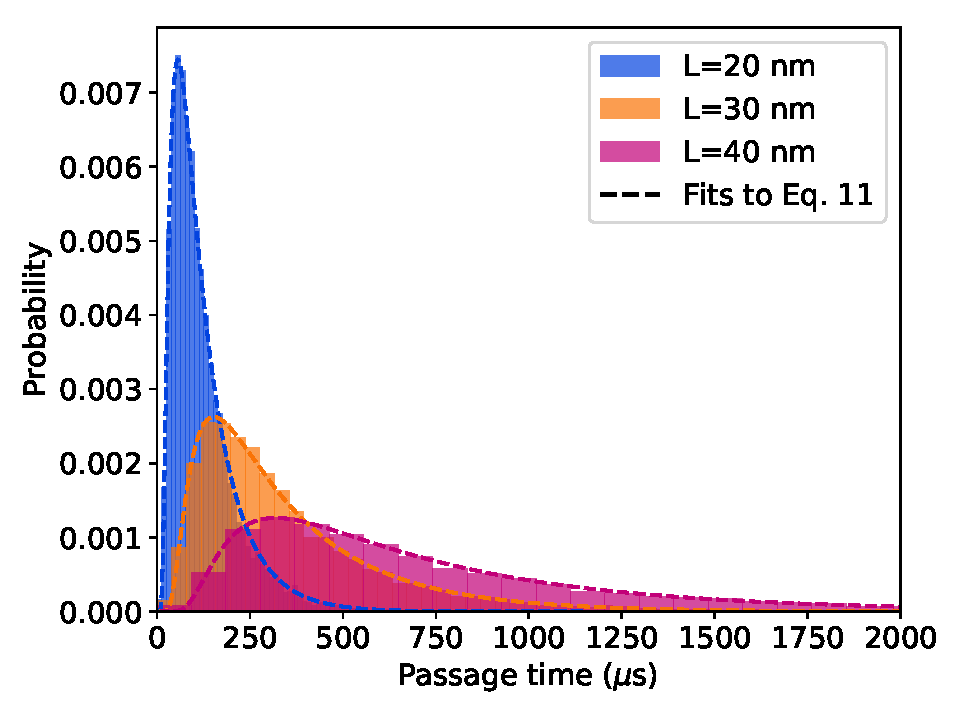
\includegraphics[width=\textwidth]{ad_fpt_distributions_URE.pdf}
  \caption{Urea}\label{fig:URE_ad_fpt_distributions}
  \end{subfigure}
  \begin{subfigure}{0.45\textwidth}
  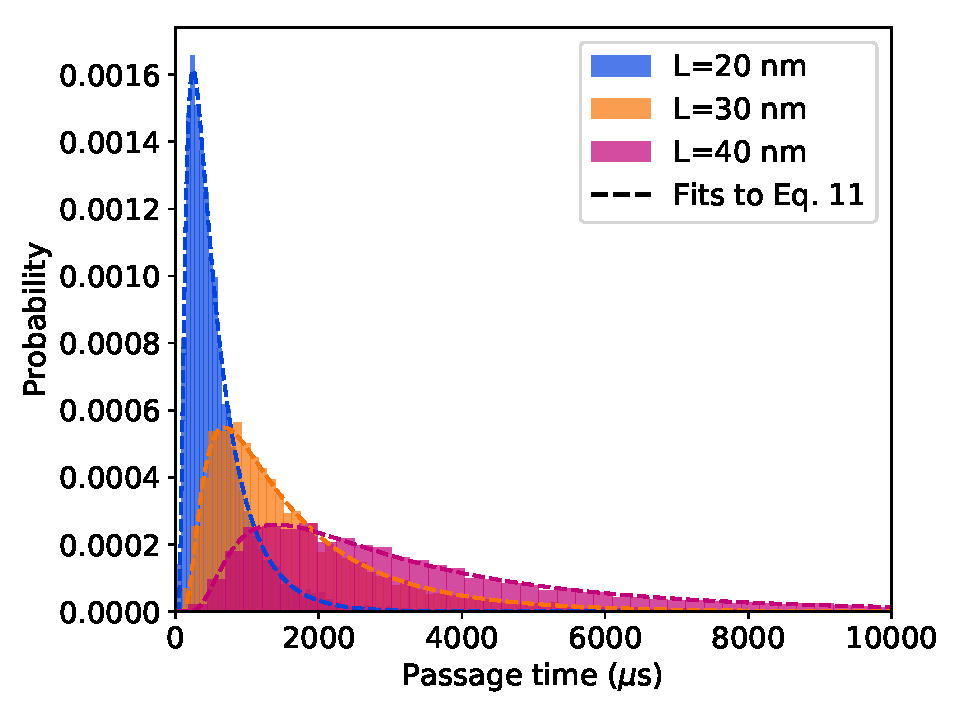
\includegraphics[width=\textwidth]{ad_fpt_distributions_ACH.pdf}
  \caption{Acetic Acid}\label{fig:ACH_ad_fpt_distributions}
  \end{subfigure}
  \begin{subfigure}{0.45\textwidth}
  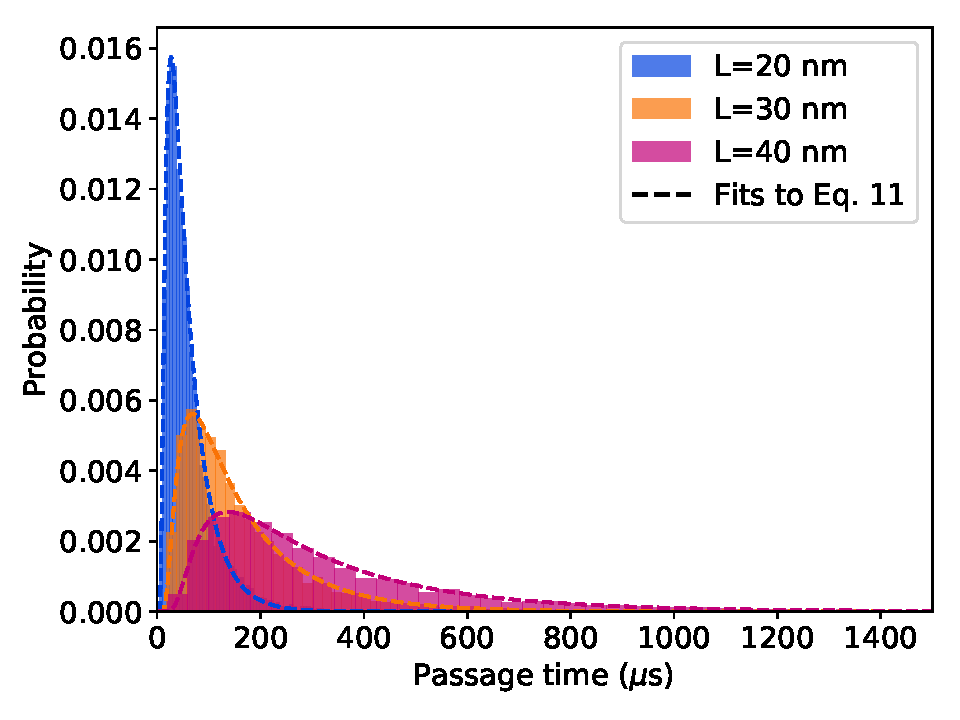
\includegraphics[width=\textwidth]{ad_fpt_distributions_GCL.pdf}
  \caption{Ethylene Glycol}\label{fig:GCL_ad_fpt_distributions}
  \end{subfigure}
  \begin{subfigure}{0.45\textwidth}
  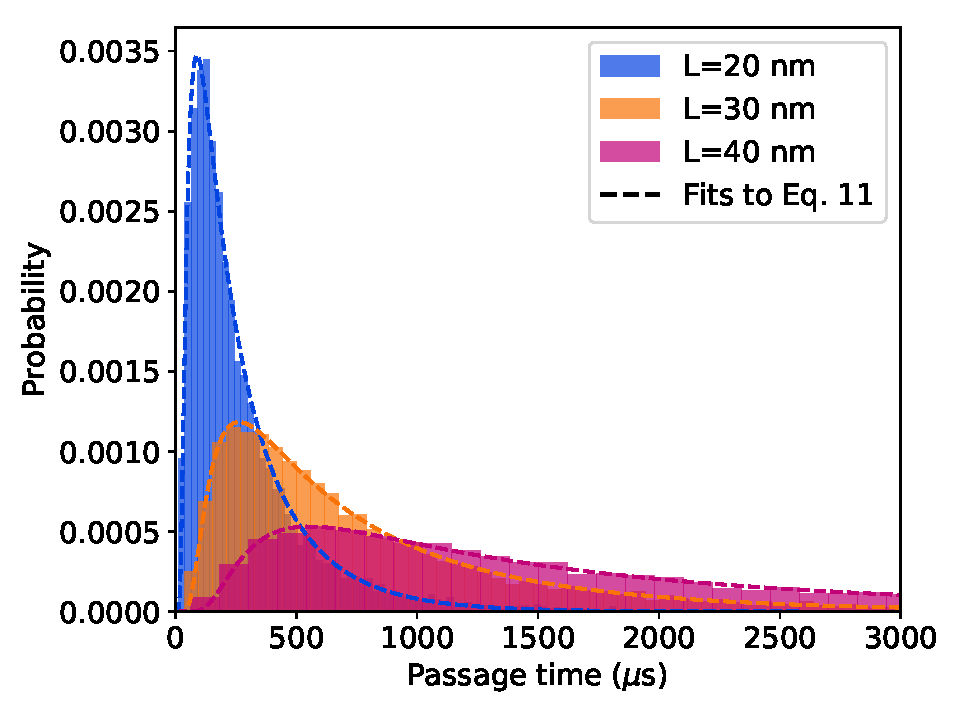
\includegraphics[width=\textwidth]{ad_fpt_distributions_MET.pdf}
  \caption{Methanol}\label{fig:MET_ad_fpt_distributions}
  \end{subfigure}
  \caption{We fit Equation~\ref{M-eqn:passage_times} of the main text to the
  first passage time distributions generated by 10,000 realizations of the 
  anomalous diffusion model. }\label{fig:ad_fpt_fits}
  \end{figure}
  
%  \begin{figure}
%  \centering
%  \begin{subfigure}{0.45\textwidth}
%  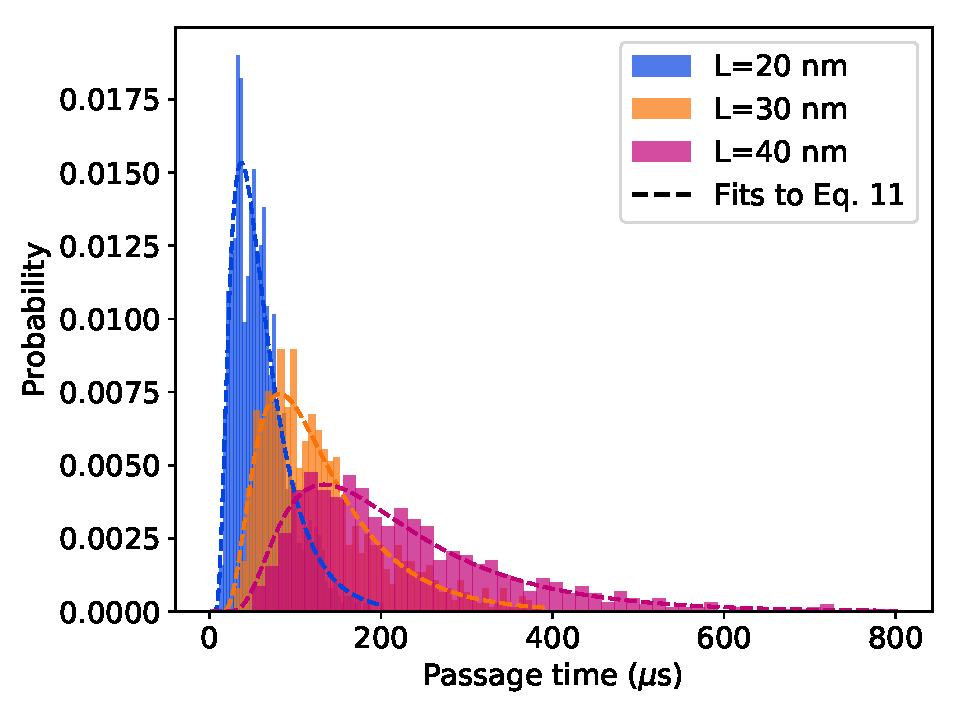
\includegraphics[width=\textwidth]{msddm_fpt_distributions_URE.pdf}
%  \caption{Urea}\label{fig:URE_msddm_fpt_distributions}
%  \end{subfigure}
%  \begin{subfigure}{0.45\textwidth}
%  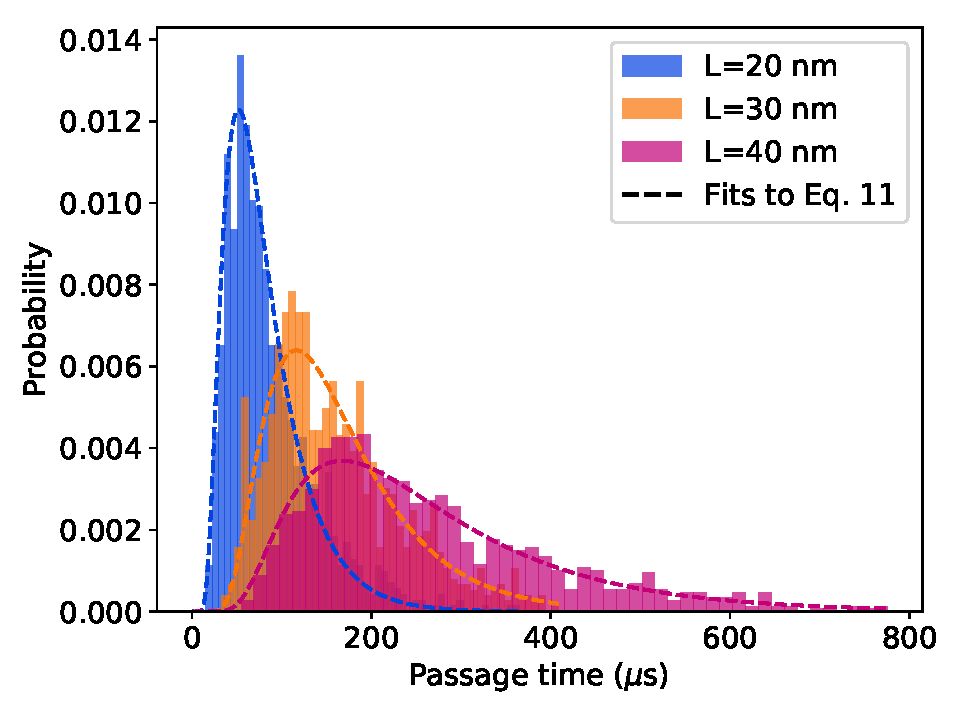
\includegraphics[width=\textwidth]{msddm_fpt_distributions_ACH.pdf}
%  \caption{Acetic Acid}\label{fig:ACH_msddm_fpt_distributions}
%  \end{subfigure}
%  \begin{subfigure}{0.45\textwidth}
%  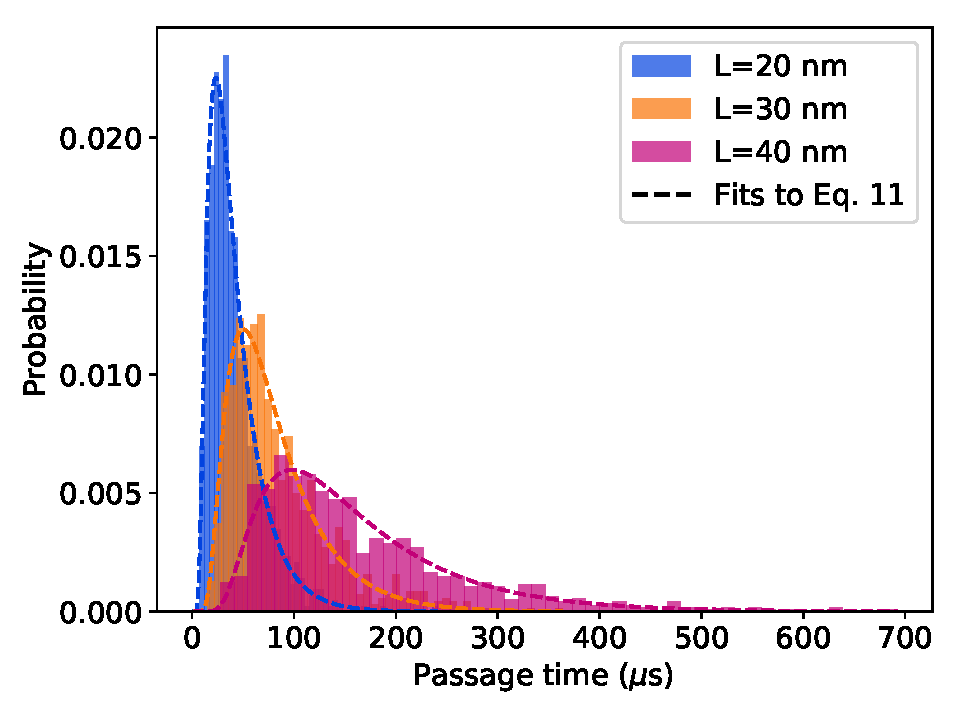
\includegraphics[width=\textwidth]{msddm_fpt_distributions_GCL.pdf}
%  \caption{Ethylene Glycol}\label{fig:GCL_msddm_fpt_distributions}
%  \end{subfigure}
%  \begin{subfigure}{0.45\textwidth}
%  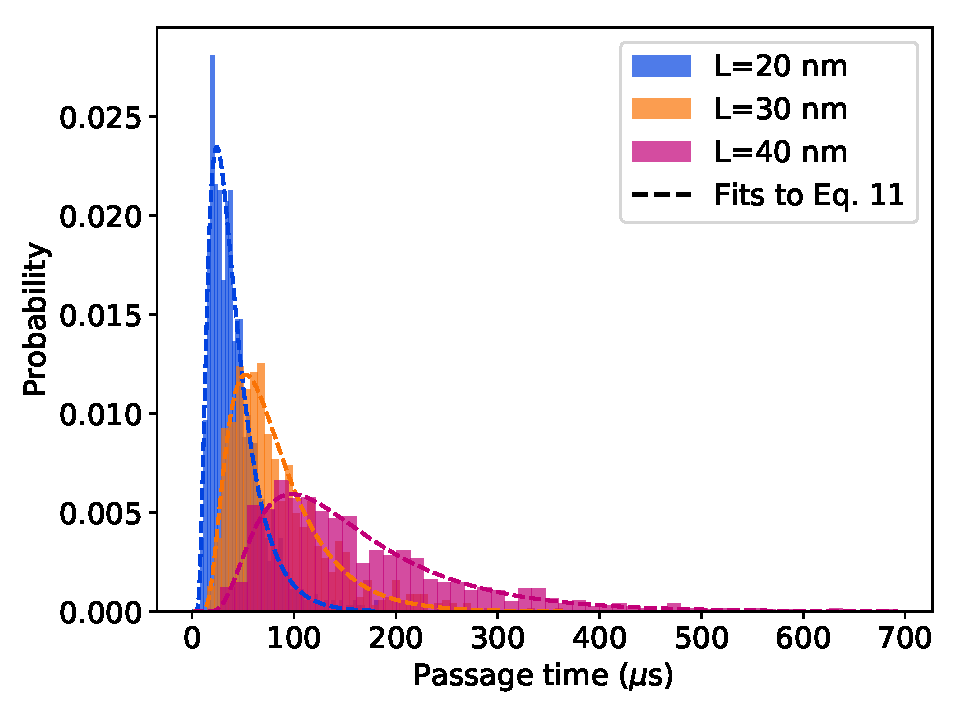
\includegraphics[width=\textwidth]{msddm_fpt_distributions_MET.pdf}
%  \caption{Methanol}\label{fig:MET_msddm_fpt_distributions}
%  \end{subfigure}
%  \caption{We fit Equation~\ref{M-eqn:passage_times} of the main text to the
%  first passage time distributions generated by 1000 realizations of the 
%  Markov state dependent dynamical model. Note that we generated 10 times less
%  realizations of the MSDDM which leads to noisier histograms. We show that
%  this has a negligible effect on the fits in Figure~\ref{fig:flux_curve_sensitivity}.}\label{fig:msddm_fpt_fits}
%  \end{figure}

%  \begin{figure}
%  \centering
%  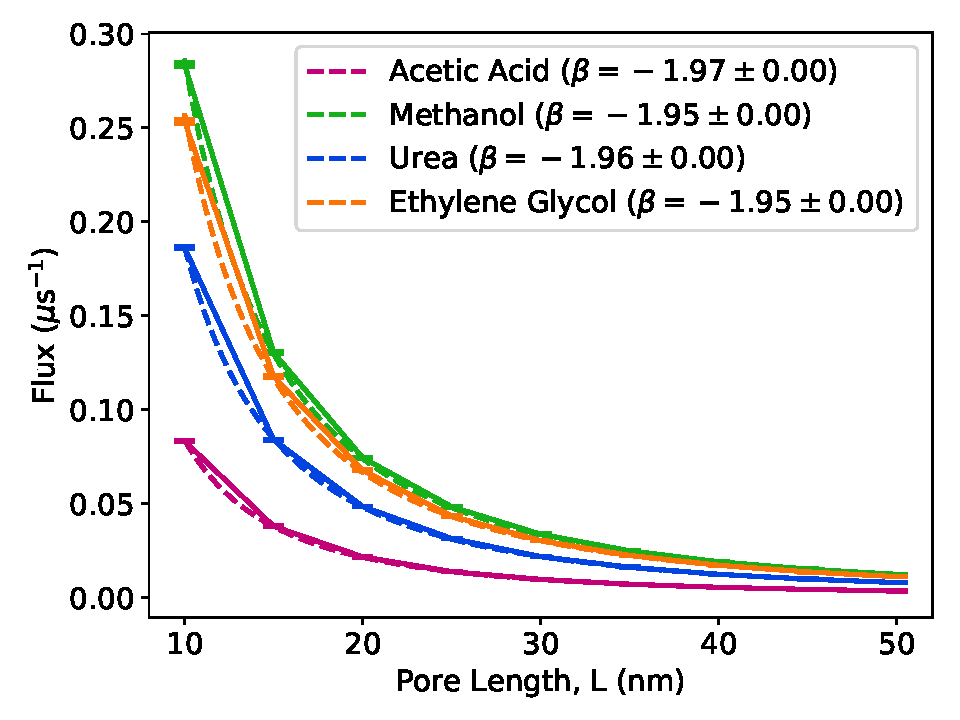
\includegraphics[width=0.5\textwidth]{flux_curves_brownian.pdf}
%  \caption{Fixed $H=0.5$}\label{fig:flux_curves_brownian}
%  \end{figure}
%  
%  \begin{figure}
%  \centering
%  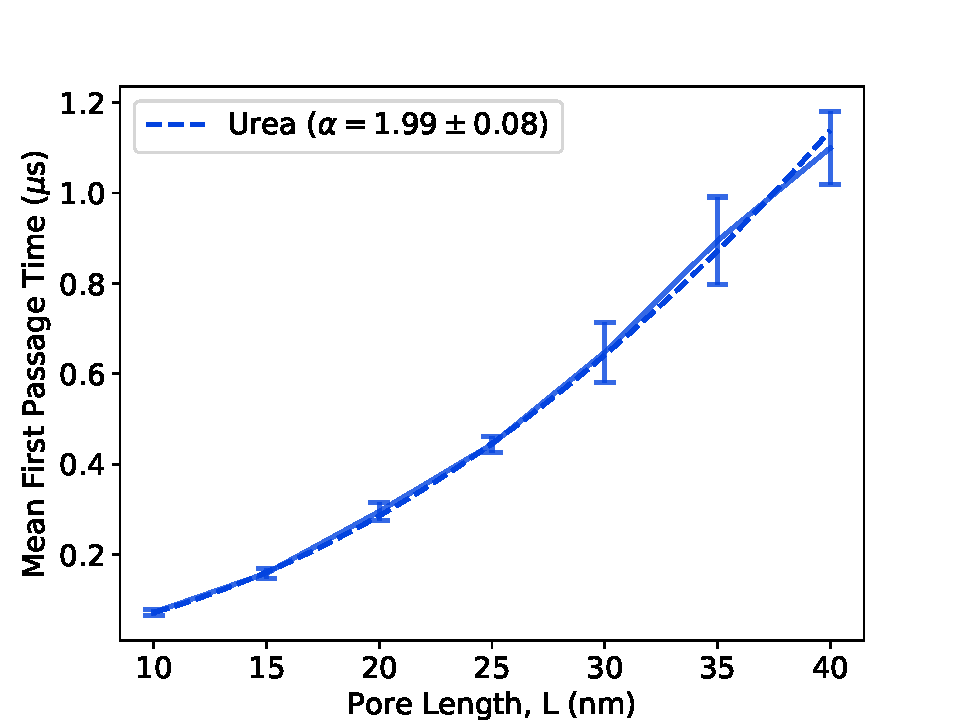
\includegraphics[width=0.45\textwidth]{mfpt_curves_brownian.pdf}
%  \caption{}\label{fig:mfpt_curve_brownian}
%  \end{figure}

  \begin{figure}
  \centering
  \begin{subfigure}{0.45\textwidth}
  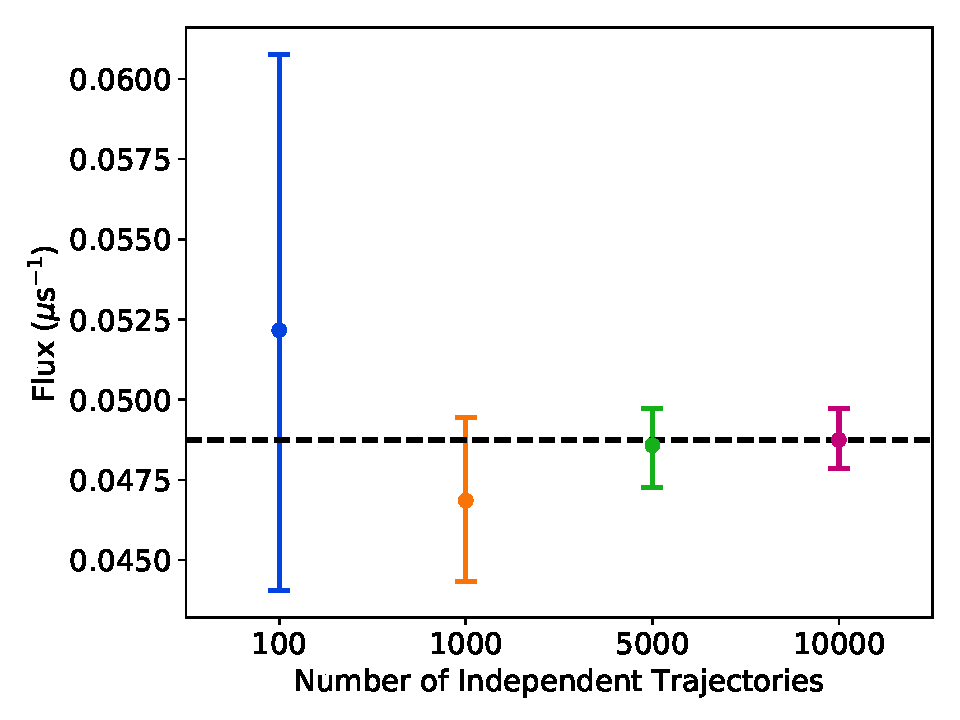
\includegraphics[width=\textwidth]{flux_curves_Nsensitivity_URE.pdf}
  \caption{urea}\label{fig:Nsensitivity_URE}
  \end{subfigure}
  \begin{subfigure}{0.45\textwidth}
  \includegraphics[width=\textwidth]{flux_curves_Nsensitivity_ACH.pdf}
  \caption{acetic acid}\label{fig:Nsensitivity_ACH}
  \end{subfigure}
  \begin{subfigure}{0.45\textwidth}
  \includegraphics[width=\textwidth]{flux_curves_Nsensitivity_GCL.pdf}
  \caption{ethylene glycol}\label{fig:Nsensitivity_GCL}
  \end{subfigure}
  \begin{subfigure}{0.45\textwidth}
  \includegraphics[width=\textwidth]{flux_curves_Nsensitivity_MET.pdf}
  \caption{methanol}\label{fig:Nsensitivity_MET}
  \end{subfigure}
  \caption{Even using a small number of independent trajectories, one can
  reliably estimate solute flux across a pore 10 nm long. The uncertainty in 
  the flux values decreases as we add more independent trajectories.
  }\label{fig:flux_curve_sensitivity}
  \end{figure}
  
  \begin{figure}
  \centering
  \begin{subfigure}{0.45\textwidth}
  \includegraphics[width=\textwidth]{flux_curves_Asensitivity_URE.pdf}
  \caption{urea}\label{fig:Asensitivity_URE}
  \end{subfigure}
  \begin{subfigure}{0.45\textwidth}
  \includegraphics[width=\textwidth]{flux_curves_Asensitivity_ACH.pdf}
  \caption{acetic acid}\label{fig:Asensitivity_ACH}
  \end{subfigure}
  \begin{subfigure}{0.45\textwidth}
  \includegraphics[width=\textwidth]{flux_curves_Asensitivity_GCL.pdf}
  \caption{ethylene glycol}\label{fig:Asensitivity_GCL}
  \end{subfigure}
  \begin{subfigure}{0.45\textwidth}
  \includegraphics[width=\textwidth]{flux_curves_Asensitivity_MET.pdf}
  \caption{methanol}\label{fig:Asensitivity_MET}
  \end{subfigure}
  \caption{The flux scaling parameter ($A$) can be reliably estimated using
  as few as 100 independent realizations of the sFBMcut AD model. To estimate
  $A$, we fit Equation~\ref{M-eqn:flux_decay} of the main text to a series of
  flux measurements made with 10, 15, 20, 25, 30, 35, 40, 45 and 50 nm pores (see
  Figure~\ref{M-fig:flux_curves_ad} of the main text).
  }\label{fig:A_sensitivity}
  \end{figure}
  
  \begin{figure}
  \centering
  \begin{subfigure}{0.45\textwidth}
  \includegraphics[width=\textwidth]{flux_curves_betasensitivity_URE.pdf}
  \caption{urea}\label{fig:betasensitivity_URE}
  \end{subfigure}
  \begin{subfigure}{0.45\textwidth}
  \includegraphics[width=\textwidth]{flux_curves_betasensitivity_ACH.pdf}
  \caption{acetic acid}\label{fig:betasensitivity_ACH}
  \end{subfigure}
  \begin{subfigure}{0.45\textwidth}
  \includegraphics[width=\textwidth]{flux_curves_betasensitivity_GCL.pdf}
  \caption{ethylene glycol}\label{fig:betasensitivity_GCL}
  \end{subfigure}
  \begin{subfigure}{0.45\textwidth}
  \includegraphics[width=\textwidth]{flux_curves_betasensitivity_MET.pdf}
  \caption{methanol}\label{fig:betasensitivity_MET}
  \end{subfigure}
  \caption{Similar to $A$, the parameter which describes the scaling of solute
  flux with pore length, $\beta$, can be reliably estimated using as few as 100
  independent realizations of the sFBMcut AD model. We estimated $\beta$ and
  $A$ simultaneously as described in Figure~\ref{fig:A_sensitivity}.
  }\label{fig:beta_sensitivity}
  \end{figure}
  
%  \begin{figure}
%  \centering
%  \begin{subfigure}{0.45\textwidth}
%  \includegraphics[width=\textwidth]{flux_curves_N100.pdf}
%  \caption{100 Independent Trajectories}\label{fig:N100}
%  \end{subfigure}
%  \begin{subfigure}{0.45\textwidth}
%  \includegraphics[width=\textwidth]{flux_curves_N1000.pdf}
%  \caption{1000 Independent Trajectories}\label{fig:N1000}
%  \end{subfigure}
%  \begin{subfigure}{0.45\textwidth}
%  \includegraphics[width=\textwidth]{flux_curves_N5000.pdf}
%  \caption{5000 Independent Trajectories}\label{fig:N5000}
%  \end{subfigure}
%  \begin{subfigure}{0.45\textwidth}
%  \includegraphics[width=\textwidth]{flux_curves_N9984.pdf}
%  \caption{10000 Independent Trajectories}\label{fig:N10000}
%  \end{subfigure}
%  \caption{Even using a small number of independent trajectories, one can
%  reliably calculate flux as a function of pore length. The uncertainty in
%  the flux curves decreases as we add more independent trajectories.}\label{fig:flux_curve_sensitivity}
%  \end{figure}
  %MRS8: is there a way to make it easier to see the fact that the data is relatively independent of length?
  %MRS8: Right now, you essentially have to scan between the 4 charts to see the numbers are about right. Maybe
  %MRS8: organize it so that the 4 charts are for 4 molecules, and each chart shows plot of 
  %MRS8: trajectory number vs pore length, so one can see that the value stays about the same except for uncertainty as 
  %MRS8: number of trajectories changes
  % equations here 
  % Analytical CDF: https://journals.aps.org/pre/pdf/10.1103/PhysRevE.73.046104
  % Analytical MFPT https://journals.aps.org/pre/pdf/10.1103/PhysRevE.62.6065
  % Figures: mfpt_pdf.pdf and mfpt_cdf.pdf

%  \newpage
%
%  \section{Explanation of Under-Estimated MSDDM $\beta$ Values}\label{section:beta_estimates}
%  
%  The value of $\beta$ for the MSDDM is under-estimated due to assumptions of the model
%  itself as well as inaccuracies in the correlation structure of very long FLM trajectories.
%  Turning first to the model itself, we have designed it to ensure that the magnitude of the
%  hops in the series of transitions between states are anti-correlated from start to finish. 
%  This assumes that the transition correlation structure is unaffected by the
%  sub-trajectories between each state transition. Each time a state transition occurs, one
%  must initialize a new time series sub-trajectory with its own correlation structure. 
%  %Even with a low Hurst parameter, as exhibited by most trapped states, the time spent 
%  %in each state is relatively short making the accuracy of the correlation structure 
%  %questionable. Additionally, $\sigma$ of transitional hops is similar in magnitude to
%  %$\sigma$ in trapped states. 
%  Since we add the transitional hop lengths to each end of
%  trapped state sub-trajectories, the transitional hop lengths are shifted with respect 
%  to one another, decreasing correlation between them. We tested this reasoning by modifying the 
%  MSDDM to completely immobilize particles except when they transition between states. 
%  Surprisingly, $\beta$ is still close to the Brownian value. Further experimentation 
%  reveals that this is actually a consequence of the FLM simulation procedure. Simulating
%  FLM requires Riemann-sum approximations of the stochastic integrals defining the process.
%  To generate the curves in Figure~\ref{M-fig:flux_curves_msddm}, we needed to correlate 
%  25--1000 times more hops than for the MSD predictions in Figure~\ref{M-fig:msddm_performance}. 
%  In short, it is computationally infeasible to use enough terms to accurately incorporate
%  long timescale correlations into our long MSDDM realizations. Thus at long timescales, 
%  we lose correlation between transitional jumps. We confirmed this hypothesis by using 
%  fractional Brownian motion, for which we have an exact simulation method, in place of 
%  FLM in the MSDDM algorithm. When we use FBM, $\beta$ increases well above the Brownian 
%  value. $\beta$ increases even further if we immobilize the trapped states. Thus the low
%  value of $\beta$ of the MSDDM is a consequence of model assumptions and inexact simulation
%  of FLM.  
%  
%  \begin{figure}[h]
%  \centering
%  \begin{subfigure}{0.43\textwidth}
%  \includegraphics[width=\textwidth]{beta_hurst.pdf}
%  \caption{}\label{fig:beta_hurst}
%  \end{subfigure}
%  \begin{subfigure}{0.52\textwidth}
%  \includegraphics[width=\textwidth]{beta_parameters.pdf}
%  \caption{}\label{fig:beta_parameters}
%  \end{subfigure}
%  %BJC5: need to update MSDDM (immobile states). Waiting on those simulations
%  %MRS6: should try to lead with what the overall results/conclusions are.  What does it mean that parameters are larger or smaller?  What should the reader take from the discussion?  Should it be in supporting?
%  \caption{(a) The $\beta$ values of the sFBMcut model appear to be inversely proportional
%  to the Hurst parameters. The $\beta$ values of the MSDDM are much lower with much less
%  variation than the sFBMcut model. (b) The $\beta$ parameters of the MSDDM are low because
%  sub-trajectories between state transitions decorrelate transitional hops and because
%  our FLM simulation procedure does not accurately correlate hops after long time lags. 
%  The high $\beta$ parameters of the sFBMcut model are a consequence of anti-correlation
%  between hops. Removing hop correlations causes $\beta$ to drop down close to MSDDM
%  values (sFBMcut ($H$=0.5)). Removing dwell times in addition to hop correlation
%  yields a similar value of $\beta$ (Brownian). Immobilizing particles while in a trapped state
%  also yields a similar value of $\beta$ (MSDDM (immobile states)). Replacing FLM with
%  FBM in the MSDDM raises $\beta$ well above the Brownian value (MSDDM (FBM)). Replacing FLM with FBM and
%  immobilizing particles in trapped states further raises the value of $\beta$.}\label{fig:beta}
%  \end{figure}

  \clearpage
  \bibliography{stochastic_transport}

\end{document}

% LocalWords:  LLC solutes py equispaced solute's ctrw sfbm ctrwsim MSD solute
% LocalWords:  MSDDM XXXX GitHub plateaued Meroz Sokolov superdiffusion MSDs wt
% LocalWords:  subdiffusion msd PR nojump xtc gro ETH nboot pdf subdiffusive xr
% LocalWords:  RWF brownian FBM CTRWs traj npt fracshow Taqqu recentering MFPT
% LocalWords:  Markovianity timestep GCL acf ACH bothmode params BJC tex acid's
% LocalWords:  sFBMcut sFLMcut urea's timescale msddm fpt CDF mfpt cdf hurst
% LocalWords:  decorrelate
